\documentclass[12pt, a4paper]{article}
\usepackage[utf8]{inputenc}
\usepackage[T2A]{fontenc}
\usepackage[russian]{babel}
\usepackage{amsmath,amsfonts,amssymb,amsthm}
\usepackage{graphicx}
\usepackage{booktabs}
\usepackage{tabularx}
\usepackage{multirow}
\usepackage{geometry}
\usepackage{setspace}
\usepackage{xcolor}
\usepackage{ragged2e}
\usepackage{listings}
\usepackage{graphicx}
\usepackage{subcaption}
\usepackage{caption}
\usepackage{indentfirst}
\usepackage{longtable}
\usepackage{enumitem}
\usepackage{hyperref}
\hypersetup{
	colorlinks=true,
	linkcolor=blue!70!black,
	citecolor=green!70!black,
	urlcolor=magenta!70!black
}


\geometry{left=2.5cm, right=1.5cm, top=2cm, bottom=2cm}
\onehalfspacing


\lstdefinestyle{mypythonstyle}{
	language=Python,
	basicstyle=\small\ttfamily,
	numbers=left,
	numberstyle=\tiny\color{gray},
	frame=tb,
	framesep=5pt,
	framerule=0.4pt,
	breaklines=true,
	keywordstyle=\color{blue}\bfseries,
	stringstyle=\color{red!80!black},
	commentstyle=\color{green!60!black}\itshape,
	identifierstyle=\color{black},
	showspaces=false,
	showtabs=false,
	showstringspaces=false,
	tabsize=2,
	captionpos=b,
	aboveskip=1.5\medskipamount,
	belowskip=\medskipamount,
	escapeinside={\%*}{*)}
}
\lstdefinestyle{mybashstyle}{
	language=bash,
	basicstyle=\small\ttfamily,
	numbers=left,
	numberstyle=\tiny\color{gray},
	frame=tb,
	framesep=5pt,
	framerule=0.4pt,
	breaklines=true,
	keywordstyle=\color{blue}\bfseries,
	stringstyle=\color{red!80!black},
	commentstyle=\color{green!60!black}\itshape,
	identifierstyle=\color{black},
	showspaces=false,
	showtabs=false,
	showstringspaces=false,
	tabsize=2,
	captionpos=b,
	aboveskip=1.5\medskipamount,
	belowskip=\medskipamount,
	escapeinside={\%*}{*)}
}
\lstdefinestyle{myjsonstyle}{
	language=json,
	basicstyle=\small\ttfamily,
	numbers=left,
	numberstyle=\tiny\color{gray},
	frame=tb,
	framesep=5pt,
	framerule=0.4pt,
	breaklines=true,
	keywordstyle=\color{blue}\bfseries,
	stringstyle=\color{red!80!black},
	commentstyle=\color{green!60!black}\itshape,
	identifierstyle=\color{black},
	showspaces=false,
	showtabs=false,
	showstringspaces=false,
	tabsize=2,
	captionpos=b,
	aboveskip=1.5\medskipamount,
	belowskip=\medskipamount,
	escapeinside={\%*}{*)}
}
\lstset{style=mypythonstyle}

\lstset{
	inputencoding=utf8, % Tell listings the input is UTF-8
	extendedchars=true,  % Allow extended characters
	literate= % Define how to display Cyrillic characters
	{а}{{\selectfont\char224}}1 {б}{{\selectfont\char225}}1 {в}{{\selectfont\char226}}1 {г}{{\selectfont\char227}}1
	{д}{{\selectfont\char228}}1 {е}{{\selectfont\char229}}1 {ё}{{\"e}}1      {ж}{{\selectfont\char230}}1
	{з}{{\selectfont\char231}}1 {и}{{\selectfont\char232}}1 {й}{{\selectfont\char233}}1 {к}{{\selectfont\char234}}1
	{л}{{\selectfont\char235}}1 {м}{{\selectfont\char236}}1 {н}{{\selectfont\char237}}1 {о}{{\selectfont\char238}}1
	{п}{{\selectfont\char239}}1 {р}{{\selectfont\char240}}1 {с}{{\selectfont\char241}}1 {т}{{\selectfont\char242}}1
	{у}{{\selectfont\char243}}1 {ф}{{\selectfont\char244}}1 {х}{{\selectfont\char245}}1 {ц}{{\selectfont\char246}}1
	{ч}{{\selectfont\char247}}1 {ш}{{\selectfont\char248}}1 {щ}{{\selectfont\char249}}1 {ъ}{{\selectfont\char250}}1
	{ы}{{\selectfont\char251}}1 {ь}{{\selectfont\char252}}1 {э}{{\selectfont\char253}}1 {ю}{{\selectfont\char254}}1
	{я}{{\selectfont\char255}}1
	{А}{{\selectfont\char192}}1 {Б}{{\selectfont\char193}}1 {В}{{\selectfont\char194}}1 {Г}{{\selectfont\char195}}1
	{Д}{{\selectfont\char196}}1 {Е}{{\selectfont\char197}}1 {Ё}{{\"E}}1      {Ж}{{\selectfont\char198}}1
	{З}{{\selectfont\char199}}1 {И}{{\selectfont\char200}}1 {Й}{{\selectfont\char201}}1 {К}{{\selectfont\char202}}1
	{Л}{{\selectfont\char203}}1 {М}{{\selectfont\char204}}1 {Н}{{\selectfont\char205}}1 {О}{{\selectfont\char206}}1
	{П}{{\selectfont\char207}}1 {Р}{{\selectfont\char208}}1 {С}{{\selectfont\char209}}1 {Т}{{\selectfont\char210}}1
	{У}{{\selectfont\char211}}1 {Ф}{{\selectfont\char212}}1 {Х}{{\selectfont\char213}}1 {Ц}{{\selectfont\char214}}1
	{Ч}{{\selectfont\char215}}1 {Ш}{{\selectfont\char216}}1 {Щ}{{\selectfont\char217}}1 {Ъ}{{\selectfont\char218}}1
	{Ы}{{\selectfont\char219}}1 {Ь}{{\selectfont\char220}}1 {Э}{{\selectfont\char221}}1 {Ю}{{\selectfont\char222}}1
	{Я}{{\selectfont\char223}}1,
	basicstyle=\small\ttfamily, % A default basic style
	breaklines=true,
	showstringspaces=false
	% Add other global settings you want for all listings
}

\lstdefinestyle{myjsonstyle}{
	% language=json, % Commented out or replaced
	language=XML, % Example replacement, or remove for plain text
	keywordstyle=\color{blue}\bfseries,
	stringstyle=\color{red!80!black},
	commentstyle=\color{green!60!black}\itshape,
	identifierstyle=\color{black},
	tabsize=2,
	captionpos=b,
	aboveskip=1.5\medskipamount,
	belowskip=\medskipamount,
	escapeinside={\%*}{*)}
}


\newtheorem{theorem}{Теорема}[section]
\newtheorem{lemma}[theorem]{Лемма}
\newtheorem{corollary}[theorem]{Следствие}
\newtheorem{proposition}{Утверждение}[section]
\theoremstyle{definition}
\newtheorem{definition}{Определение}[section]
\newtheorem{example}{Пример}[section]
\theoremstyle{remark}
\newtheorem{remark}{Замечание}[section]


\addto\captionsrussian{%
	\renewcommand{\figurename}{Рис.}%
	\renewcommand{\tablename}{Табл.}%
	\renewcommand{\lstlistingname}{Листинг}%
}
\renewcommand{\contentsname}{Содержание}

\title{Проект по дисциплине: \\ «Анализ изображений и компьютерное зрение» \\ FrameReader}
\author{Команда «Пришли пить кофе»}
\date{\today}

\begin{document}
	
	\maketitle
	\thispagestyle{empty}
	\newpage
	\tableofcontents
	\newpage
	\setcounter{page}{1}
	
	\section{Введение}
	\subsection{Описание проблемы}
	Наш проект FrameReader направлен на решение актуальной задачи автоматического извлечения и распознавания текстовой информации из видеопотоков. В современном мире объем видеоконтента постоянно растет, и ручной анализ каждого кадра на предмет наличия текста становится неэффективным и трудозатратным. Мы видим острую потребность в автоматизации этого процесса.
	
	\subsection{Зачем это нужно (потенциальные пользователи, кейсы применения)}
	Автоматическое извлечение текста из видео является критически важным для множества прикладных задач. Мы выделяем следующие ключевые кейсы применения и потенциальных пользователей:
	\begin{itemize}
		\item \textbf{Медиа-компании и контент-платформы:} Для индексации видеоконтента, автоматического создания субтитров, поиска по тексту внутри видео, мониторинга упоминаний брендов или ключевых слов в новостных сюжетах и рекламных материалах.
		\item \textbf{Маркетинговые агентства:} Для анализа эффективности рекламных кампаний, отслеживания размещения логотипов и текстовых сообщений в видеорекламе конкурентов.
		\item \textbf{Службы безопасности и видеонаблюдения:} Для автоматического распознавания номерных знаков, вывесок, предупреждающих надписей в видеопотоках с камер наблюдения.
		\item \textbf{Разработчики систем видеоаналитики:} Для интеграции функционала OCR в более сложные системы анализа поведения, событий или объектов в видео.
		\item \textbf{Образовательные учреждения:} Для индексации лекций и вебинаров, позволяя студентам быстро находить нужную информацию по тексту на слайдах или доске.
	\end{itemize}
	Наш проект предоставляет мощный инструмент для автоматизации этих процессов, значительно сокращая время и ресурсы, необходимые для анализа видеоконтента.
	
	\subsection{Постановка задачи}
	Основная задача, которую мы ставим перед проектом FrameReader, заключается в разработке комплексного и высокоэффективного решения для:
	\begin{enumerate}
		\item \textbf{Детекции текстовых областей на кадрах видео:} Точное определение местоположения и размеров текстовых блоков.
		\item \textbf{Распознавания текста (OCR) из выделенных областей:} Преобразование изображений текстовых блоков в машиночитаемый текст.
		\item \textbf{Предоставления удобного интерфейса для взаимодействия с системой и просмотра результатов:} Разработка интуитивно понятного пользовательского интерфейса для загрузки видео, мониторинга процесса обработки и визуализации полученных данных.
		\item \textbf{Обеспечения масштабируемости и производительности решения для обработки больших объемов данных:} Создание архитектуры, способной эффективно обрабатывать значительные объемы видеоконтента с минимальными задержками.
	\end{enumerate}
	Для решения этой задачи мы используем современные методы компьютерного зрения и машинного обучения. В качестве данных для обучения моделей мы активно используем датасет \href{https://www.kaggle.com/datasets/hardtype/rustitw-russian-language-visual-text-recognition}{RusTitW}, содержащий изображения русского текста, что позволяет нам достигать высокой точности для нашей целевой аудитории.
	
	\subsection{Стек технологий}
	Мы построили проект FrameReader на современном и эффективном стеке технологий, который обеспечивает гибкость, производительность и масштабируемость каждого компонента системы.
	
	\bigskip
	\noindent
	\begin{tabularx}{\textwidth}{|l|>{\RaggedRight\arraybackslash}X|}
		\toprule
		\textbf{Ветка} & \textbf{Используемые технологии} \\
		\midrule
		\textbf{Server} & Python, FastAPI, WebSocket, MySQL \\
		\midrule
		\textbf{Client} & React, Chakra UI, Axios, Rutube-player \\
		\midrule
		\textbf{Train} & YOLOv12 (детекция текста), Donut (OCR), TrOCR (OCR) \\
		\midrule
		\textbf{Triton Server} & NVIDIA Triton Inference Server, Ray Serve, Docker \\
		\bottomrule
	\end{tabularx}
	
	\subsection{Этапы работы}
	Работа над проектом FrameReader была структурирована и выполнена в соответствии со следующими основными этапами:
	\begin{enumerate}
		\item \textbf{Подготовка данных:} Мы осуществили сбор, тщательный анализ, предобработку и аугментацию датасета, чтобы обеспечить высокое качество обучающих данных.
		\item \textbf{Разработка моделей:} Мы выбрали оптимальные архитектуры и провели настройку гиперпараметров для достижения наилучших результатов.
		\item \textbf{Реализация и обучение:} Мы разработали код для обучения моделей и провели серию экспериментов для их оптимизации.
		\item \textbf{Оценка качества моделей:} Мы рассчитали ключевые метрики и провели детальный анализ ошибок для каждой модели.
		\item \textbf{Развертывание системы:} Мы настроили сервер инференса, разработали бэкенд и фронтенд, обеспечив их бесперебойное взаимодействие.
		\item \textbf{Тестирование и демонстрация:} Мы провели всестороннее тестирование комплексного решения и подготовили демонстрационные материалы для наглядной презентации его возможностей.
	\end{enumerate}
	
	\section{Обзор существующих решений}
	\subsection{Общие подходы и алгоритмы к OCR в видео}
	Для детекции и распознавания текста в видео существует множество подходов. Традиционные методы, такие как комбинация алгоритмов обработки изображений (например, MSER для выделения текстовых областей) и классических OCR-движков (например, Tesseract), часто страдают от низкой точности и производительности в условиях реального видео (размытие, движение, различные шрифты и освещение).
	
	Мы сосредоточились на современных подходах, основанных на глубоком обучении. Для детекции текста широко используются архитектуры, такие как YOLO (You Only Look Once), SSD (Single Shot MultiBox Detector) и Faster R-CNN. Для распознавания текста (OCR) популярны модели на основе трансформеров, такие как TrOCR и Donut, которые показывают высокую точность даже на сложных изображениях.
	
	\subsection{Анализ рынка и конкурентная среда}
	Наш проект FrameReader решает задачу извлечения и распознавания текста из видеопотоков и функционирует в активно развивающейся области компьютерного зрения. На рынке существует ряд компаний, платформ и технологий, предлагающих аналогичные или пересекающиеся решения.
	
	\subsubsection{Основные категории конкурентов}
	
	\paragraph{1. Крупные облачные провайдеры}
	Эти компании предлагают мощные и масштабируемые API-сервисы для OCR, включая функционал для видео. Их решения часто являются «черным ящиком» с точки зрения используемых моделей, но обеспечивают высокую надежность и простоту интеграции.
	
	\begin{itemize}
		\item \textbf{Google Cloud Vision AI:}
		\begin{itemize}
			\item \textbf{Описание:} Предоставляет API для анализа изображений и видео, включая детекцию и распознавание текста. Использует предобученные модели машинного обучения.
			\item \textbf{Конкурентное преимущество:} Высокая масштабируемость, надежность, интеграция с другими сервисами Google Cloud.
			\item \textbf{Аналог FrameReader:} Прямой конкурент в части предоставления OCR-функционала для видео.
		\end{itemize}
		\item \textbf{Amazon Rekognition:}
		\begin{itemize}
			\item \textbf{Описание:} Сервис компьютерного зрения от AWS, предлагающий детекцию текста в изображениях и видео.
			\item \textbf{Конкурентное преимущество:} Глубокая интеграция в экосистему AWS, масштабируемость.
			\item \textbf{Аналог FrameReader:} Аналогичен Google Cloud Vision в контексте OCR из видео.
		\end{itemize}
		\item \textbf{Azure Cognitive Services (Computer Vision):}
		\begin{itemize}
			\item \textbf{Описание:} Набор API для компьютерного зрения от Microsoft Azure, включающий OCR для печатного и рукописного текста в изображениях и видео.
			\item \textbf{Конкурентное преимущество:} Интеграция с Azure, поддержка различных языков.
			\item \textbf{Аналог FrameReader:} Аналогичен другим облачным решениям.
		\end{itemize}
	\end{itemize}
	
	\paragraph{2. Специализированные платформы и инструменты}
	Эти компании фокусируются на предоставлении более специализированных решений или инструментов для разработчиков в области компьютерного зрения и OCR.
	
	\begin{itemize}
		\item \textbf{Sieve:}
		\begin{itemize}
			\item \textbf{Описание:} Платформа, которая занимается сравнением и предоставлением лучших методов OCR на видео, используя современные AI-модели (например, Gemini, Florence 2).
			\item \textbf{Конкурентное преимущество:} Фокус на передовых моделях, возможно, более гибкие настройки для специфических задач.
			\item \textbf{Аналог FrameReader:} Прямой конкурент, предлагающий готовые решения для видео-OCR.
		\end{itemize}
		\item \textbf{Roboflow:}
		\begin{itemize}
			\item \textbf{Описание:} Платформа для создания, аннотирования, обучения и развертывания моделей компьютерного зрения. Предоставляет инструменты для работы с OCR на видео, включая возможность аннотирования видеокадров.
			\item \textbf{Конкурентное преимущество:} Комплексный цикл разработки моделей, удобные инструменты для разметки данных.
			\item \textbf{Аналог FrameReader:} Конкурент в части обучения и развертывания моделей, а также предоставления инструментов для работы с видео.
		\end{itemize}
		\item \textbf{Panopto:}
		\begin{itemize}
			\item \textbf{Описание:} Платформа для управления видеоконтентом, которая включает функции «умного» поиска по видео, используя ASR (автоматическое распознавание речи) и OCR для индексации.
			\item \textbf{Конкурентное преимущество:} Комплексное решение для корпоративного видео, интеграция ASR и OCR для поиска.
			\item \textbf{Аналог FrameReader:} Конкурент в более широком смысле, если FrameReader будет развиваться в сторону индексации и поиска по видео.
		\end{itemize}
		\item \textbf{DENKnet (IDS Imaging):}
		\begin{itemize}
			\item \textbf{Описание:} Специализированное программное обеспечение для OCR с использованием AI, ориентированное на промышленные и специфические задачи.
			\item \textbf{Конкурентное преимущество:} Высокая точность для узкоспециализированных задач, кастомизация.
			\item \textbf{Аналог FrameReader:} Конкурент в нишевых применениях OCR.
		\end{itemize}
	\end{itemize}
	
	\paragraph{3. Открытые библиотеки и фреймворки (для самостоятельной реализации)}
	Многие разработчики создают собственные решения, используя доступные библиотеки.
	\begin{itemize}
		\item \textbf{Tesseract OCR:}
		\begin{itemize}
			\item \textbf{Описание:} Один из самых популярных открытых OCR-движков. Может использоваться для распознавания текста на отдельных кадрах видео.
			\item \textbf{Конкурентное преимущество:} Бесплатность, гибкость, широкое сообщество.
			\item \textbf{Аналог FrameReader:} Базовый инструмент, который может быть частью более сложного решения, как в случае с tesseract.js в нашей клиентской части FrameReader.
		\end{itemize}
		\item \textbf{OpenCV, FFmpeg:}
		\begin{itemize}
			\item \textbf{Описание:} Библиотеки для обработки изображений и видео, используемые для извлечения кадров, предобработки и других операций.
			\item \textbf{Конкурентное преимущество:} Фундаментальные инструменты для работы с медиа.
			\item \textbf{Аналог FrameReader:} Мы используем подобные инструменты как компоненты в нашей системе.
		\end{itemize}
		\item \textbf{PyTorch, TensorFlow, Hugging Face Transformers, Ultralytics YOLO:}
		\begin{itemize}
			\item \textbf{Описание:} Фреймворки и библиотеки для машинного обучения, позволяющие разрабатывать и обучать собственные модели детекции и распознавания текста.
			\item \textbf{Конкурентное преимущество:} Полный контроль над моделями, возможность глубокой кастомизации.
			\item \textbf{Аналог FrameReader:} Это те самые инструменты, на которых построен FrameReader.
		\end{itemize}
	\end{itemize}
	
	\subsubsection{Позиционирование проекта FrameReader}
	FrameReader, с его архитектурой, включающей обучение кастомных моделей, использование Triton Server для инференса, а также собственный бэкенд и фронтенд, позиционируется как комплексное, кастомизируемое решение для OCR из видео с акцентом на русский язык. Ключевые конкурентные преимущества FrameReader заключаются в:
	\begin{itemize}
		\item Оптимизации под русский язык: Мы проводим специализированное обучение моделей на русскоязычных данных.
		\item Гибкости развертывания: Мы обеспечиваем возможность развертывания на собственном оборудовании с использованием Triton Server.
		\item Контроле над всем пайплайном: Мы контролируем весь процесс от обучения моделей до пользовательского интерфейса.
		\item Возможности интеграции: Мы предоставляем API для легкой интеграции в другие системы.
	\end{itemize}
	Таким образом, FrameReader занимает нишу между полностью облачными «черными ящиками» и полностью самописными решениями на базе открытых библиотек, предлагая баланс между готовым функционалом и возможностью глубокой кастомизации.
	
	\subsubsection{Сравнительный анализ: преимущества и недостатки FrameReader}
	Благодаря нашей специализации и архитектуре, FrameReader занимает уникальное положение на рынке решений для оптического распознавания текста (OCR) из видео.
	
	\paragraph{Преимущества FrameReader:}
	\begin{itemize}
		\item \textbf{Глубокая кастомизация и оптимизация под русский язык:}
		Мы обучаем и оптимизируем модели (YOLO, Donut, TrOCR) специально на русскоязычных данных (например, RusTitW). Это позволяет нам достичь значительно более высокой точности и релевантности для русского текста по сравнению с универсальными моделями. Большинство крупных облачных OCR-сервисов предлагают общие модели, которые могут не обеспечивать оптимального качества для русского языка.
		\item \textbf{Полный контроль над пайплайном (от обучения до развертывания):}
		FrameReader охватывает весь жизненный цикл моделей машинного обучения: от подготовки данных и обучения до оптимизации (TensorRT, квантизация), развертывания (NVIDIA Triton Inference Server, Ray Serve) и предоставления пользовательского интерфейса. Это дает нам полный контроль над каждым этапом. Облачные API ограничивают прозрачность и контроль.
		\item \textbf{Высокая производительность инференса:}
		Использование NVIDIA Triton Inference Server, Ray Serve и наша оптимизация моделей (TensorRT, квантизация) обеспечивают высокую пропускную способность и низкую задержку. Это критично для обработки больших объемов видео или работы в реальном времени. Open-source решения могут быть менее оптимизированы, а облачные сервисы дорогими при больших объемах.
		\item \textbf{Гибкость развертывания (On-Premise):}
		Мы обеспечиваем возможность развертывания всего решения на собственной инфраструктуре (on-premise) с использованием Docker. Это важно для организаций со строгими требованиями к безопасности данных или желающих избежать зависимости от облачных провайдеров.
		\item \textbf{Комплексное решение с открытым исходным кодом (частично):}
		FrameReader предоставляет достаточно открытых компонентов для понимания внутренней работы, адаптации или расширения, что не всегда возможно с проприетарными решениями.
	\end{itemize}
	
	\paragraph{Недостатки FrameReader:}
	\begin{itemize}
		\item \textbf{Сложность развертывания и поддержки:}
		Развертывание и поддержка такого комплексного решения, как FrameReader, требует значительных технических знаний, опыта в DevOps и ML, а также вычислительных ресурсов. Это не «коробочное» решение. Облачные сервисы предлагают более простой процесс интеграции.
		\item \textbf{Отсутствие готовой инфраструктуры и SLA:}
		В настоящее время FrameReader не поставляется с готовой, управляемой инфраструктурой, гарантированной доступностью (SLA) и круглосуточной поддержкой. Эти аспекты ложатся на команду, развертывающую решение. Облачные сервисы это гарантируют.
		\item \textbf{Высокие первоначальные затраты на разработку и обучение:}
		Разработка наших кастомных моделей и создание всей инфраструктуры требует значительных первоначальных инвестиций времени и ресурсов. Готовые API позволяют начать работу быстро с оплатой по мере использования.
		\item \textbf{Ограниченная мультиязычность «из коробки»:}
		Хотя FrameReader оптимизирован под русский язык, поддержка других языков потребует с нашей стороны дополнительного обучения и адаптации моделей. Многие облачные решения предлагают широкую мультиязычную поддержку сразу.
		\item \textbf{Меньшая известность и экосистема:}
		Будучи относительно новым проектом, FrameReader пока не имеет такой широкой экосистемы, сообщества и готовых интеграций, как крупные игроки рынка. Крупные платформы имеют обширную документацию и активное сообщество.
	\end{itemize}
	
	\subsubsection{Итоговый вывод по конкурентному анализу}
	FrameReader идеально подходит для компаний или проектов, которым требуется высокоточный и специализированный OCR для русского языка с возможностью глубокой кастомизации и развертывания на собственной инфраструктуре. Мы предлагаем мощный и гибкий инструментарий для тех, кто готов инвестировать в развертывание, поддержку и дальнейшее развитие нашего решения.
	
	Для пользователей, которым нужна максимально простая интеграция, готовое решение «из коробки» и не критична специфическая оптимизация под русский язык или полный контроль над моделями, облачные API или специализированные платформы могут быть более предпочтительными.
	
	\subsection{Обоснование выбора методов в проекте FrameReader}
	Мы выбрали YOLOv12 для детекции текста, так как его высокая скорость и точность критичны для обработки видео в реальном времени. Для OCR мы остановили свой выбор на моделях Donut и TrOCR благодаря их способности эффективно работать с различными типами текста и документов, а также их возможностям для оптимизации под инференс. TrOCR хорошо зарекомендовал себя в задачах end-to-end OCR, в то время как Donut предлагает гибкость для понимания документов и может быть адаптирован для извлечения структурированной информации, что мы рассматриваем как перспективное направление для развития FrameReader.
	
	\section{Подготовка данных}
	\subsection{Описание выбранного датасета}
	Для обучения моделей детекции и распознавания текста в нашем проекте FrameReader мы используем датасет \href{https://www.kaggle.com/datasets/hardtype/rustitw-russian-language-visual-text-recognition}{RusTitW (Russian Language Visual Text Recognition)}. Этот датасет, разработанный Игорем Марковым, Сергеем Нестеруком, Андреем Кузнецовым и Денисом Димитровым (подробнее в \href{https://arxiv.org/abs/2303.16531}{arXiv:2303.16531}), содержит изображения русского текста в естественных условиях (in-the-wild), что полностью соответствует основной задаче нашего проекта. Данные в RusTitW разделены на обучающую (train) и тестовую (test) выборки, каждая из которых, в свою очередь, содержит как реальные, так и синтетические (synth) примеры. Для удобства использования, каждая папка с данными сопровождается файлом \texttt{info.csv}, имеющим единый формат для всех частей датасета. Оригинальные метки и информация также сохранены и доступны в файлах \texttt{info\_raw.csv} или \texttt{json\_*\_*.json}. Стоит отметить, что в датасете присутствуют дубликаты изображений (например, одинаковые изображения с разным разрешением) и некоторое пересечение изображений между обучающей и тестовой выборками, что унаследовано из оригинальных источников данных.
	
	Изначально, метки в датасете RusTitW представлены в формате JSON, описывающем ограничивающие рамки (bounding boxes) и соответствующий им текст. Пример такой метки:
	\begin{lstlisting}[basicstyle=\small\ttfamily\linespread{0.9}, numbers=none, frame=none, aboveskip=1ex, belowskip=1ex]
		[[{'left': 0.10259433962264151,
			'top': 0,
			'width': 0.4056603773584906,
			'height': 0.9303675048355899,
			'label': 'ALL you NEED\nis 20 SECONDS\nof Insane',
			'shape': 'rectangle'},
		... % другие рамки
		]]
	\end{lstlisting}
	Здесь \texttt{left}, \texttt{top}, \texttt{width}, \texttt{height} — относительные координаты и размеры рамки, а \texttt{label} — текст внутри нее.
	
	\subsection{Предобработка данных}
	Процесс предобработки данных в нашем проекте включает несколько ключевых этапов:
	\begin{itemize}
		\item \textbf{Нормализация:} Приведение изображений к стандартному размеру, например, 640x640 пикселей для модели детекции YOLO и 384x384 пикселей для моделей распознавания Donut и TrOCR.
		\item \textbf{Очистка:} Удаление некорректных или плохо аннотированных данных для повышения качества обучающей выборки.
		\item \textbf{Аугментация:} Применение различных преобразований к изображениям (повороты, масштабирование, изменение яркости/контрастности, добавление шума). Это позволяет увеличить разнообразие обучающей выборки и повысить устойчивость моделей к вариациям во входных данных, что способствует лучшей генерализации моделей на новые данные.
		\item \textbf{Конвертация формата для модели Donut:} Поскольку модель Donut требует специфическую структуру данных для обучения, мы выполняем конвертацию датасета RusTitW в требуемый формат. Это включает организацию данных в следующую иерархию директорий:
		
		\begin{lstlisting}[basicstyle=\small\ttfamily\linespread{0.9}, numbers=none, frame=none, aboveskip=1ex, belowskip=1ex]
			dataset_name/
			+-- test/
			|   +-- metadata.jsonl
			|   +-- {image_path0}
			|   L-- ...
			+-- train/
			|   +-- metadata.jsonl
			|   +-- {image_path0}
			|   L-- ...
			L-- validation/
			+-- metadata.jsonl
			+-- {image_path0}
			L-- ...
		\end{lstlisting}
		Каждый файл \texttt{metadata.jsonl} содержит строки в формате JSON, где каждая строка описывает одно изображение и его разметку:
		\begin{lstlisting}[basicstyle=\small\ttfamily\linespread{0.9}, numbers=none, frame=none, aboveskip=1ex, belowskip=1ex]
			{"file_name": "{image_path0}", "ground_truth": "{\"gt_parse\": {ground_truth_parse}, ... }"}
		\end{lstlisting}
		Для задачи чтения текста (Text Reading Task), которая также является задачей предварительного обучения модели Donut, поле \texttt{gt\_parse} имеет вид: 
		\begin{lstlisting}[basicstyle=\small\ttfamily\linespread{0.9}, numbers=none, frame=none, aboveskip=1ex, belowskip=1ex]
			|{"text_sequence" : "word1 word2 word3 ... "}|
		\end{lstlisting}
		Для генерации синтетических данных в этом формате также может быть использован инструмент SynthDoG, описанный в репозитории Donut.
	\end{itemize}
	
	\subsection{Визуализация ключевых аспектов данных}
	Для лучшего понимания характера данных, используемых в нашем проекте, ниже представлены примеры изображений из датасета RusTitW. Мы показываем как синтетические примеры, так и изображения из реальных условий.
	
	\begin{figure}[h!]
		\centering
		\includegraphics[width=0.9\textwidth]{synth.png}
		\caption{Примеры синтетических изображений из датасета RusTitW, используемых для обучения моделей.}
		\label{fig:synth_examples}
	\end{figure}
	
	\begin{figure}[h!]
		\centering
		\includegraphics[width=0.9\textwidth]{real.png}
		\caption{Примеры реальных изображений ("in-the-wild") из датасета RusTitW, демонстрирующие разнообразие текстовых сцен.}
		\label{fig:real_examples}
	\end{figure}
	
	\section{Разработка модели}
	\subsection{Используемые алгоритмы и архитектуры}
	В проекте FrameReader используются две основные категории моделей: для детекции текста и для распознавания текста.
	
	\subsubsection{Детеция текста: YOLOv12}
	Для детекции текстовых областей используется модель YOLOv12. YOLO (You Only Look Once) — это семейство моделей для обнаружения объектов в реальном времени. YOLOv12 является одной из последних итераций, предлагающей улучшенную точность и скорость.
	
	\textbf{Принцип работы YOLO:}
	YOLO делит входное изображение на сетку. Каждая ячейка сетки предсказывает ограничивающие рамки (bounding boxes) и вероятности классов для объектов, центры которых попадают в эту ячейку. Одновременно предсказываются координаты рамки $(x, y, w, h)$, где $(x, y)$ — центр рамки, $w$ — ширина, $h$ — высота, а также вероятность наличия объекта (objectness score) и вероятности классов.
	
	\begin{figure}[h!]
		\centering
		% \includegraphics[width=0.8\textwidth]{yolo_detection_example.png} % Placeholder image
		% % Файл изображения yolo_detection_example.png не предоставлен. Раскомментируйте \includegraphics и укажите путь к файлу.
		\caption{Пример детекции текста с помощью YOLOv12}
		\label{fig:yolo_detection}
	\end{figure}
	
	\subsubsection{Распознавание текста (OCR): TrOCR}
	TrOCR (Transformer-based Optical Character Recognition) — это модель, основанная на архитектуре трансформера, разработанная Microsoft для оптического распознавания символов. Она использует подход "end-to-end", то есть принимает изображение на вход и выдает текст на выход, без необходимости в промежуточных шагах, таких как сегментация символов.
	
	\textbf{Архитектура TrOCR:}
	TrOCR состоит из двух основных частей:
	\begin{itemize}
		\item \textbf{Визуальный трансформер-энкодер:} Преобразует входное изображение в последовательность признаков.
		\item \textbf{Текстовый трансформер-декодер:} Генерирует последовательность символов (текст) на основе признаков, полученных от энкодера.
	\end{itemize}
	Модель обучается как seq2seq задача, где вход — изображение, а выход — последовательность символов.
	
	\begin{figure}[h!]
		\centering
		% \includegraphics[width=0.8\textwidth]{trocr_example.png} % Placeholder image
		% % Файл изображения trocr_example.png не предоставлен. Раскомментируйте \includegraphics и укажите путь к файлу.
		\caption{Пример работы TrOCR}
		\label{fig:trocr_example}
	\end{figure}
	
	\subsubsection{Распознавание текста (OCR): Donut}
	Donut (Document Understanding Transformer) — это еще одна трансформер-модель, разработанная для понимания документов. В отличие от TrOCR, Donut ориентирован на более сложные задачи, такие как извлечение информации из форм или таблиц, но также может использоваться для общего OCR.
	
	\textbf{Особенности Donut:}
	\begin{itemize}
		\item \textbf{Не требует OCR-движка:} Donut напрямую преобразует изображение в структурированный вывод (например, JSON), минуя промежуточный этап распознавания текста.
		\item \textbf{Гибкость:} Может быть адаптирован для различных задач понимания документов.
	\end{itemize}
	
	\subsection{Обоснование выбора методов}
	Выбор конкретных архитектур (YOLOv12, TrOCR, Donut) подробно обсуждался в разделе \ref{ssec:обоснование_выбора_методов_обзор} (Обзор существующих решений). Ключевыми факторами являются высокая производительность YOLOv12 для детекции в реальном времени и передовые возможности трансформерных архитектур TrOCR и Donut для качественного распознавания текста, включая сложные случаи и возможность работы без традиционных OCR-движков.
	\label{ssec:обоснование_выбора_методов_разработка}
	
	\subsection{Гиперпараметры и стратегия обучения}
	Ниже представлены ключевые гиперпараметры и детали стратегии обучения, использованные для каждой из моделей в нашем проекте.
	
	\subsubsection{YOLOv12}
	Для обучения модели детекции текста YOLOv12 мы использовали следующие настройки:
	\begin{itemize}
		\item \textbf{Основные параметры модели и данных:}
		\begin{itemize}
			\item Размер входного изображения: 640x640 пикселей.
			\item Задача: детекция одного класса (single\_cls: true).
		\end{itemize}
		\item \textbf{Параметры процесса обучения:}
		\begin{itemize}
			\item Количество эпох: 4.
			\item Размер пакета (Batch size): автоматический подбор (\texttt{batch: -1}).
			\item Оптимизатор: (\texttt{optimizer: SGD}).
			\item Начальная скорость обучения (Learning rate, \texttt{lr0}): 0.01.
			\item Конечный фактор скорости обучения (Learning rate factor, \texttt{lrf}): 0.01.
			\item Моментум: 0.937.
			\item Регуляризация (Weight decay): 0.0005.
			\item Эпохи разогрева (Warmup epochs): 3.0.
			\item Моментум на этапе разогрева: 0.8.
			\item Скорость обучения для смещений (bias) на этапе разогрева: 0.1.
			\item Использование смешанного режима точности (AMP): включено (\texttt{amp: true}).
			\item Завершение аугментации типа "mosaic" за N последних эпох (\texttt{close\_mosaic}): 0 (т.е. mosaic не используется до конца).
		\end{itemize}
		\item \textbf{Аугментации данных (во время обучения):}
		\begin{itemize}
			\item Автоматическая аугментация: \texttt{randaugment}.
			\item Изменение цветового пространства HSV: H (\texttt{hsv\_h}: 0.015), S (\texttt{hsv\_s}: 0.7), V (\texttt{hsv\_v}: 0.4).
			\item Геометрические преобразования:
			\begin{itemize}
				\item Повороты (\texttt{degrees}): 0 (отключены в данном конфиге, но \texttt{randaugment} может применять).
				\item Сдвиг (\texttt{translate}): 0.1.
				\item Масштабирование (\texttt{scale}): 0.5.
				\item Сдвиг с наклоном (\texttt{shear}): 0.0.
				\item Перспектива (\texttt{perspective}): 0.0.
			\end{itemize}
			\item Горизонтальное отражение (\texttt{fliplr}): вероятность 0.5.
			\item Вертикальное отражение (\texttt{flipud}): вероятность 0.0.
			\item Аугментация Mosaic: вероятность 1.0.
			\item Аугментация MixUp: вероятность 0.0 (отключена).
			\item Случайное стирание (\texttt{erasing}): вероятность 0.4.
			\item Copy-Paste аугментация: вероятность 0.0 (отключена).
		\end{itemize}
		\item \textbf{Прочее:}
		\begin{itemize}
			\item Устройство для обучения: GPU 0 (\texttt{device: '0'}).
			\item Количество рабочих процессов для загрузки данных (\texttt{workers}): 8.
			\item Начальное значение для генератора случайных чисел (\texttt{seed}): 42.
			\item Детерминированный режим: включен (\texttt{deterministic: true}).
		\end{itemize}
	\end{itemize}
	
	\subsubsection{TrOCR}
	Для обучения модели распознавания текста TrOCR мы использовали следующие настройки:
	\begin{itemize}
		\item \textbf{Основные параметры модели и данных:}
		\begin{itemize}
			\item Размер входного изображения: 384x384 пикселей.
		\end{itemize}
		\item \textbf{Параметры процесса обучения:}
		\begin{itemize}
			\item Количество эпох: 5.
			\item Размер пакета (Batch size): 32.
			\item Скорость обучения (Learning rate): 5e-5.
			\item Точность вычислений (Precision): \texttt{bf16}.
		\end{itemize}
		\item \textbf{Аугментации данных:}
		\begin{itemize}
			\item Те же, что и для Donut
		\end{itemize}
		\item \textbf{Оптимизации памяти/скорости:}
		\begin{itemize}
			\item Заморозка энкодера: использовалась опция \texttt{--freeze\_encoder}.
			\item Использование Flash Attention: применялась опция \texttt{--flash\_attention}.
			\item Накопление градиента: применялась опция \texttt{--gradient\_accumulation\_steps}.
		\end{itemize}
	\end{itemize}
	
	\subsubsection{Donut}
	Для обучения модели распознавания текста Donut (дообучение на основе \texttt{Akajackson/donut\_rus} мы использовали следующие настройки:
	\begin{itemize}
		\item \textbf{Основные параметры модели и данных:}
		\begin{itemize}
			\item Исходная модель: \texttt{Akajackson/donut\_rus}.
			\item Размер входного изображения: 384x384 пикселей.
			\item Максимальная длина генерируемой последовательности: 64 токена.
			\item Стартовый токен задачи: \texttt{<s\_500k>}.
			\item Конечный токен промпта: \texttt{<s\_prompt>}.
		\end{itemize}
		\item \textbf{Параметры процесса обучения:}
		\begin{itemize}
			\item Количество эпох: 25.
			\item Размер пакета (Batch size): 80.
			\item Скорость обучения (Learning rate): 5e-5.
			\item Регуляризация (Weight decay): 0.005.
			\item Доля эпох для разогрева (Warmup ratio): 0.005.
			\item Шаги накопления градиента (Gradient Accumulation Steps): 16.
			\item Максимальная норма градиента (Max grad norm): 100.0.
			\item Точность вычислений (Precision): \texttt{bf16}.
		\end{itemize}
		\item \textbf{Аугментации данных:}
		\begin{itemize}
			\item Применение аугментаций: включено (\texttt{apply\_augmentation: true}).
			\item Вероятность применения аугментации: 0.3 (\texttt{augmentation\_prob}).
			\item Максимальный угол поворота: $\pm$8.0 градусов (\texttt{max\_rotation}).
			\item Диапазон яркости: [0.8, 1.2] (\texttt{brightness\_min}, \texttt{brightness\_max}).
			\item Диапазон контрастности: [0.8, 1.2] (\texttt{contrast\_min}, \texttt{contrast\_max}).
			\item Диапазон размытия (blur kernel size): [0, 2] (\texttt{blur\_min}, \texttt{blur\_max}).
			\item Уровень шума: 0.05 (\texttt{noise\_level}).
			\item Диапазон резкости: [0.8, 1.5] (\texttt{sharpness\_min}, \texttt{sharpness\_max}).
		\end{itemize}
		\item \textbf{Прочее:}
		\begin{itemize}
			\item Устройство для обучения: \texttt{cuda}.
			\item Количество рабочих процессов для загрузки данных (\texttt{num\_workers}): 8.
			\item Ранняя остановка (Early stopping): терпение 60 шагов (\texttt{early\_stopping\_patience}), порог 0.1 (\texttt{early\_stopping\_threshold}).
		\end{itemize}
	\end{itemize}
	
	\section{Реализация и обучение}
	\subsection{Описание кода и окружения}
	\subsubsection{Окружение и фреймворки}
	\begin{itemize}
		\item \textbf{Python:} Версия 3.10 и выше.
		\item \textbf{GPU:} Рекомендуется NVIDIA GPU (например, A100 80GB) для эффективного обучения.
		\item \textbf{CUDA:} Версия 12.1 и выше.
		\item \textbf{Фреймворки:} PyTorch, Hugging Face Transformers, Ultralytics YOLO.
	\end{itemize}
	
	\subsubsection{Структура кода и скрипты обучения}
	Обучение моделей YOLOv12, TrOCR и Donut производится с использованием соответствующих скриптов и Jupyter-ноутбуков, доступных в ветке $train$ репозитория.
	\begin{itemize}
		\item \textbf{Ветка $train$:} Отвечает за обучение, оптимизацию и подготовку моделей компьютерного зрения. Содержит все необходимые скрипты, конфигурации и инструменты.
		\item \textbf{YOLOv12:} Обучение осуществляется с использованием Jupyter-ноутбуков в директории $train/notebooks$. Скрипты для обучения и инференса также находятся в директории $train\_yolo$. Обученные модели экспортируются в формат TensorRT через $model.export(format='engine')$.
		\item \textbf{TrOCR:} Обучение производится с использованием скрипта $train\_trocr/train.py$.
		\item \textbf{Donut:} Обучение осуществляется с использованием скрипта $train\_donut/train.py$. Для Donut предусмотрены специальные скрипты для экспорта в TensorRT.
	\end{itemize}
	
	\subsection{Процесс обучения}
	Точное время обучения зависит от используемого оборудования (GPU), размера датасета и выбранных гиперпараметров. Учитывая использование A100 GPU и оптимизированных фреймворков, обучение моделей занимает разумное время. Но, разумное в рамках практики глубокого обучения, мы модель не дообучили, полное обучение заняло примерно 14 часов для модели Donut и примерно 10 часов для модели Yolo.
	
	\subsubsection{YOLOv12}
	\begin{itemize}
		\item \textbf{Метрики качества (во время обучения):}
		Динамика изменения ключевых метрик и потерь в процессе обучения модели YOLOv12 представлена на рисунке \ref{fig:yolo_results_plot}. Таблица \ref{tab:yolo_metrics_summary} содержит сводку этих метрик для четырех эпох обучения.
		
		\begin{figure}[h!]
			\centering
			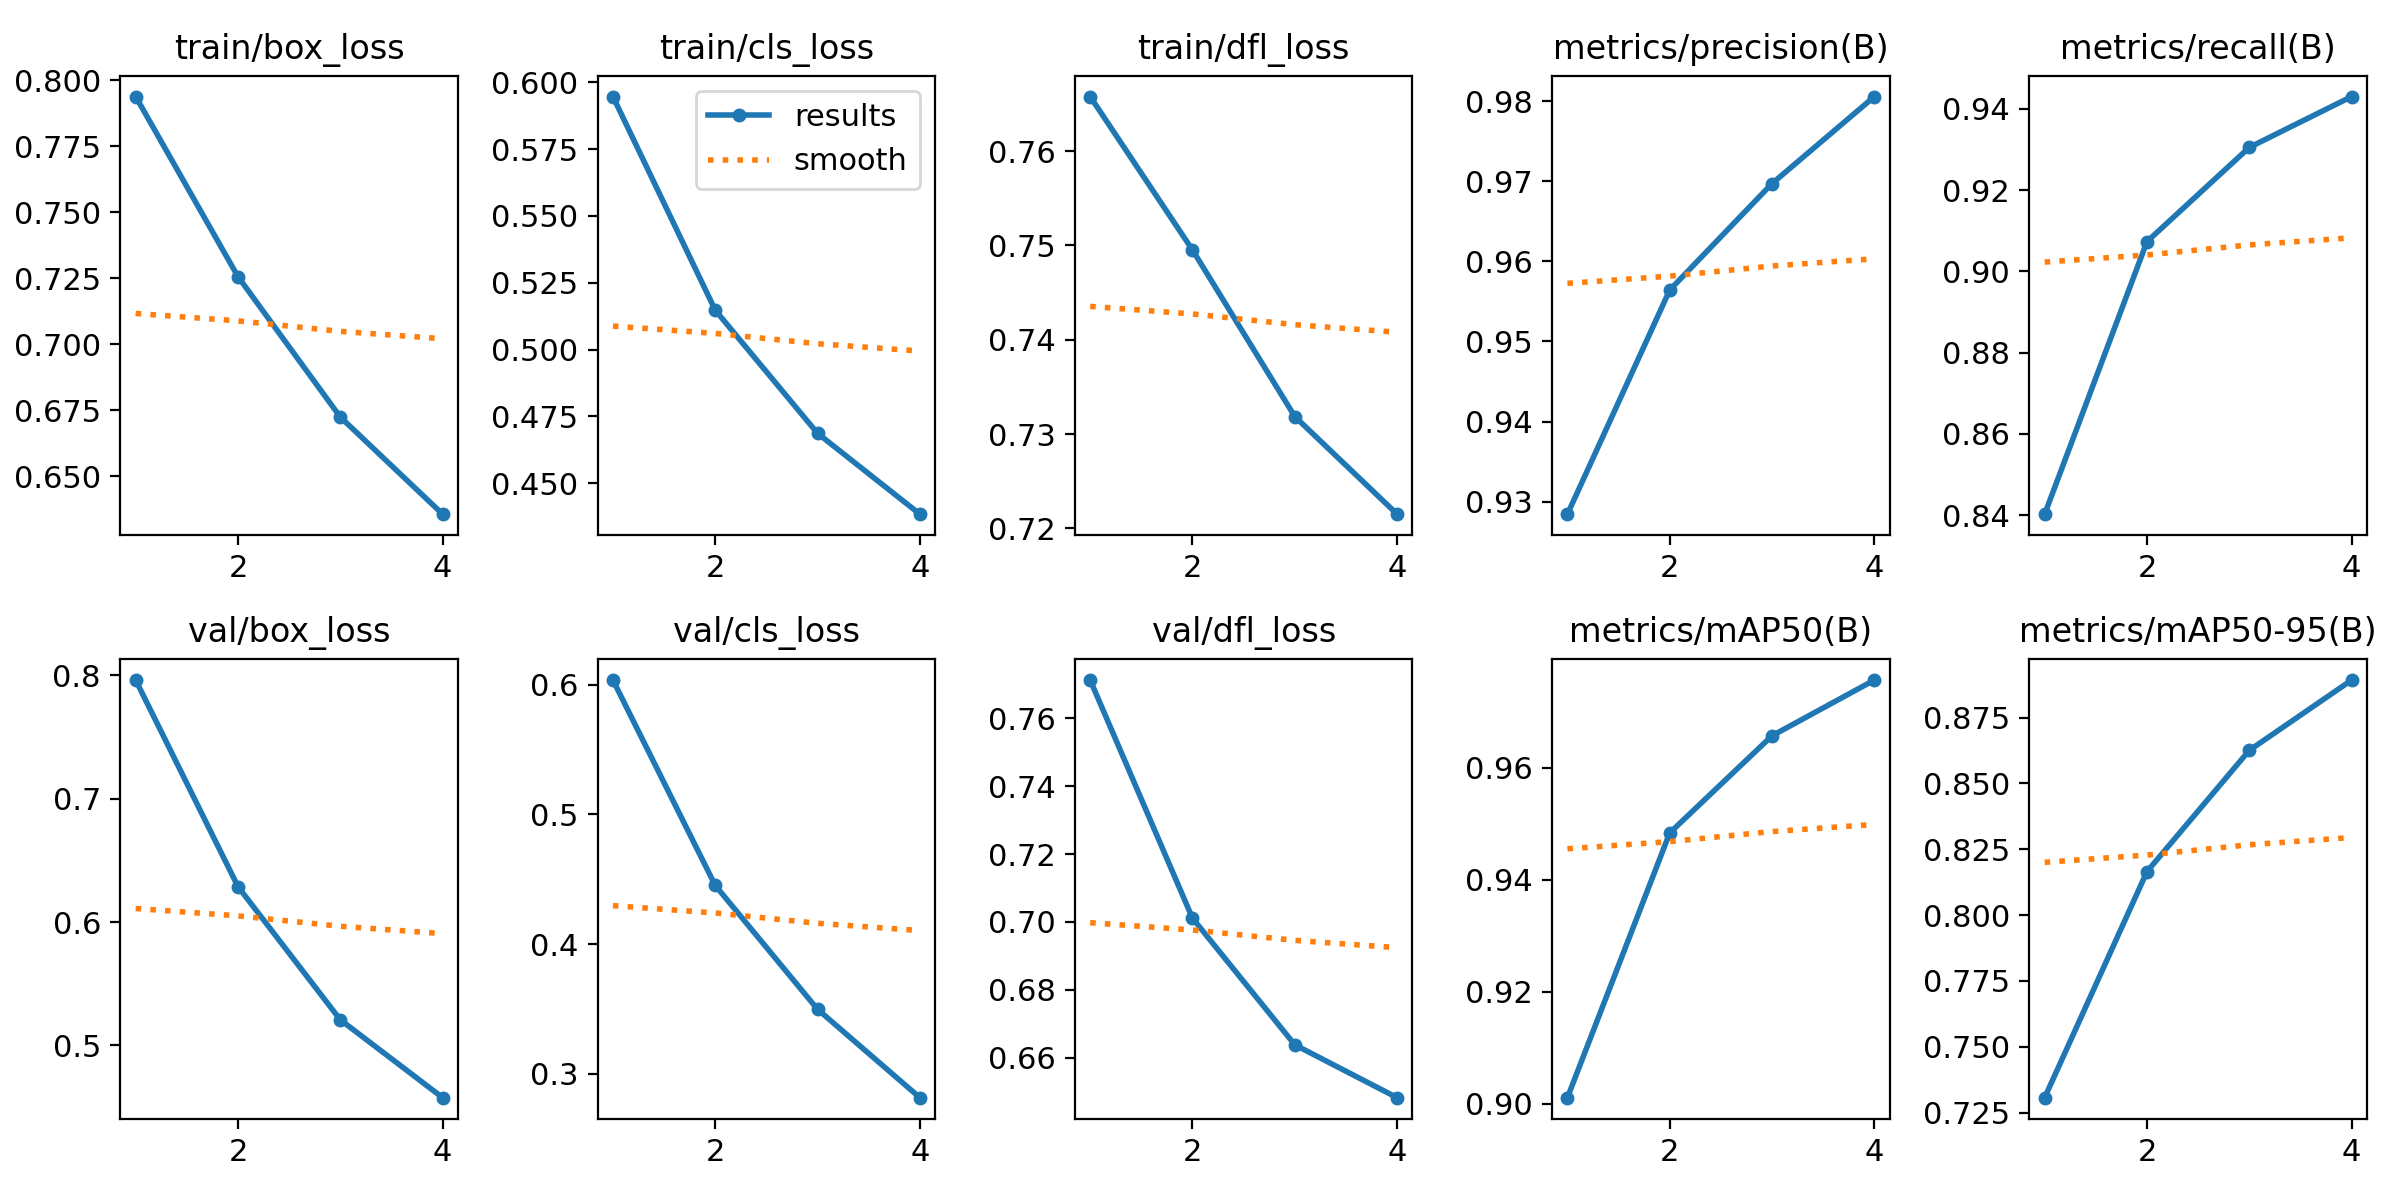
\includegraphics[width=\textwidth]{results.png}
			\caption{Графики метрик и потерь обучения модели YOLOv12.}
			\label{fig:yolo_results_plot}
		\end{figure}
		
		\begin{table}[h!]
			\centering
			\caption{Сводка метрик обучения YOLOv12 (первые 4 эпохи).}
			\label{tab:yolo_metrics_summary}
			\resizebox{\textwidth}{!}{
				\begin{tabular}{@{}lcccc@{}}
					\toprule
					\textbf{Метрика} & \textbf{Эпоха 1} & \textbf{Эпоха 2} & \textbf{Эпоха 3} & \textbf{Эпоха 4} \\
					\midrule
					Время эпохи (сек) & 2125.79 & 2207.64 & 2155.75 & 2140.18 \\
					\midrule
					\multicolumn{5}{l}{\textit{Потери на обучающей выборке (Train Loss)}} \\
					\quad train/box\_loss & 0.79375 & 0.72553 & 0.67236 & 0.63558 \\
					\quad train/cls\_loss & 0.59467 & 0.51476 & 0.4687 & 0.43846 \\
					\quad train/dfl\_loss & 0.76579 & 0.74952 & 0.73185 & 0.7215 \\
					\midrule
					\multicolumn{5}{l}{\textit{Метрики на валидационной выборке (Validation Metrics)}} \\
					\quad metrics/precision(B) & 0.92845 & 0.95642 & 0.96971 & 0.98056 \\
					\quad metrics/recall(B) & 0.84026 & 0.90733 & 0.93051 & 0.94302 \\
					\quad metrics/mAP50(B) & 0.90105 & 0.94836 & 0.96571 & 0.97566 \\
					\quad metrics/mAP50-95(B) & 0.73067 & 0.81653 & 0.86257 & 0.88925 \\
					\midrule
					\multicolumn{5}{l}{\textit{Потери на валидационной выборке (Validation Loss)}} \\
					\quad val/box\_loss & 0.79622 & 0.62871 & 0.52074 & 0.45762 \\
					\quad val/cls\_loss & 0.60364 & 0.44523 & 0.34971 & 0.28156 \\
					\quad val/dfl\_loss & 0.77125 & 0.70109 & 0.66379 & 0.64822 \\
					\midrule
					\multicolumn{5}{l}{\textit{Скорость обучения (Learning Rate)}} \\
					\quad lr/pg0 & 0.074136 & 0.048258 & 0.022375 & 0.010447 \\
					\quad lr/pg1 & 0.003025 & 0.006049 & 0.009068 & 0.010447 \\
					\quad lr/pg2 & 0.003025 & 0.006049 & 0.009068 & 0.010447 \\
					\bottomrule
				\end{tabular}
			}
		\end{table}
	\end{itemize}
	
	\subsubsection{TrOCR}
	Пример команды для обучения:
	\begin{lstlisting}[style=mybashstyle, caption=Пример команды обучения TrOCR]
		python train_trocr/train.py \
		--data_dir path/to/dataset \
		--output_dir ./trocr_output \
		--batch_size 32 \
		--precision bf16 \
		--image_size 384 384 \
		--learning_rate 5e-5 \
		--num_epochs 10
	\end{lstlisting}
	\begin{itemize}
		\item \textbf{Метрики качества (во время обучения):}
		Динамика изменения потерь на обучающей выборке в процессе обучения модели TrOCR представлена на рисунке \ref{fig:trocr_metrics_plot}. Таблица \ref{tab:trocr_metrics_summary} содержит сводку этих потерь, скорости обучения и времени на эпоху для первых пяти эпох.
		
		\begin{figure}[h!]
			\centering
			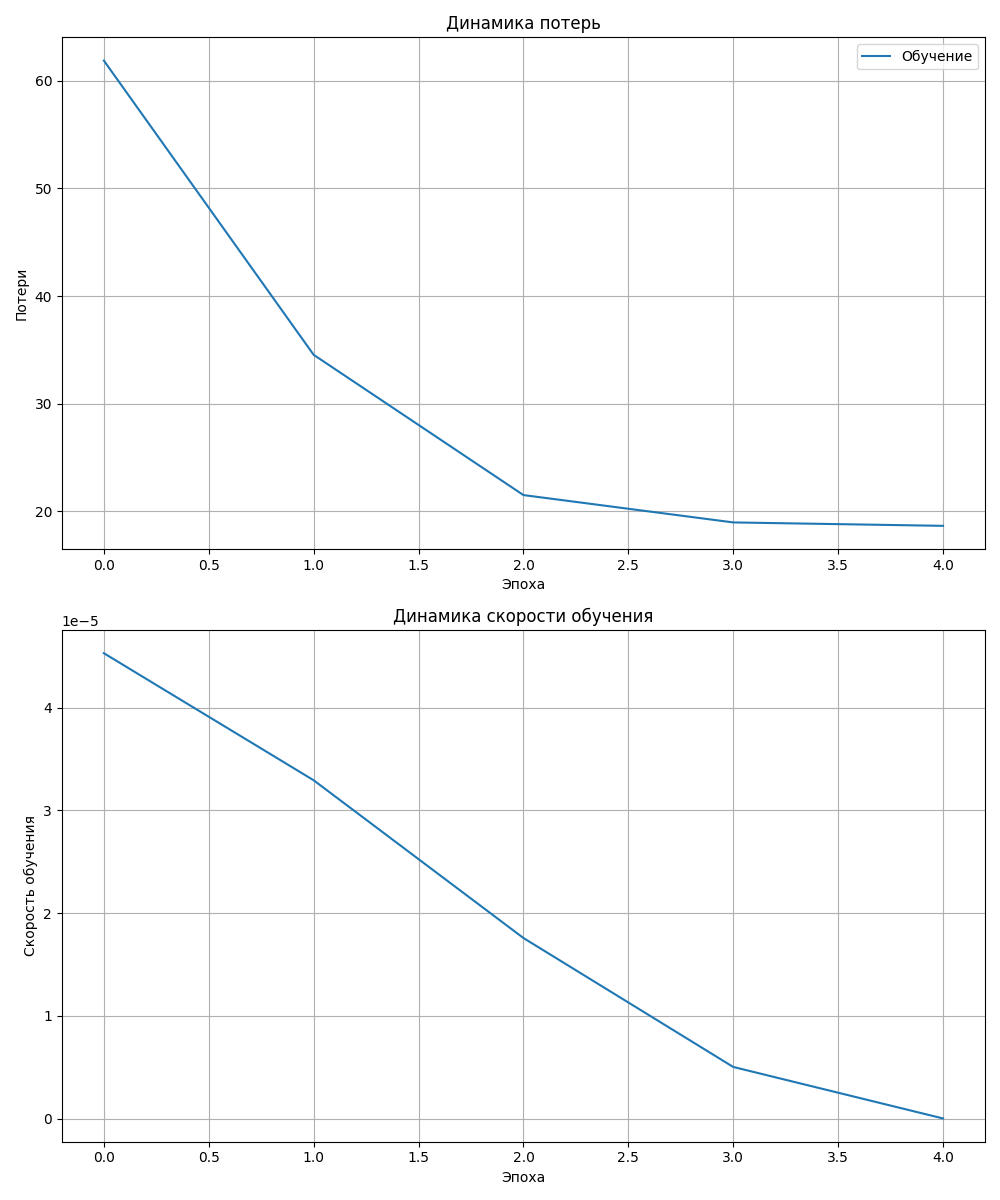
\includegraphics[width=0.8\textwidth]{metrics_epoch_5.png}
			\caption{График потерь обучения модели TrOCR (первые 5 эпох).}
			\label{fig:trocr_metrics_plot}
		\end{figure}
		
		\begin{table}[h!]
			\centering
			\caption{Сводка метрик обучения TrOCR (первые 5 эпох).}
			\label{tab:trocr_metrics_summary}
			\begin{tabular}{@{}lccccc@{}}
				\toprule
				\textbf{Метрика / Эпоха} & \textbf{1} & \textbf{2} & \textbf{3} & \textbf{4} & \textbf{5} \\
				\midrule
				Train Loss & 61.8813 & 34.5386 & 21.5036 & 18.9625 & 18.6446 \\
				Learning Rate & 4.53e-05 & 3.29e-05 & 1.76e-05 & 5.02e-06 & 5.24e-09 \\
				Time per Epoch (s) & 7139.92 & 7166.27 & 7161.35 & 7166.90 & 7168.94 \\
				\bottomrule
			\end{tabular}
		\end{table}
	\end{itemize}
	
	\subsubsection{Donut}
	Пример команды для обучения:
	\begin{lstlisting}[style=mybashstyle, caption=Пример команды обучения Donut]
		python train_donut/train.py \
		--data_dir path/to/documents \
		--output_dir ./donut_output \
		--batch_size 80 \
		--image_size 384 384 \
		--apply_augmentation \
		--num_epochs 30 
	\end{lstlisting}
	\begin{itemize}
		\item \textbf{Метрики качества (во время обучения):}
		Динамика изменения потерь на обучающей и валидационной выборках в процессе обучения модели Donut представлена на рисунке \ref{fig:donut_metrics_plot}. Таблица \ref{tab:donut_metrics_summary} содержит сводку этих потерь, скорости обучения и времени на эпоху для выбранных эпох. 
		На 5-й эпохе наблюдается значительный скачок потерь и существенное уменьшение времени на эпоху, так как сначала Donut обучалась на синтетических данных, а затем тюнилась на реальных.
		
		\begin{figure}[h!]
			\centering
			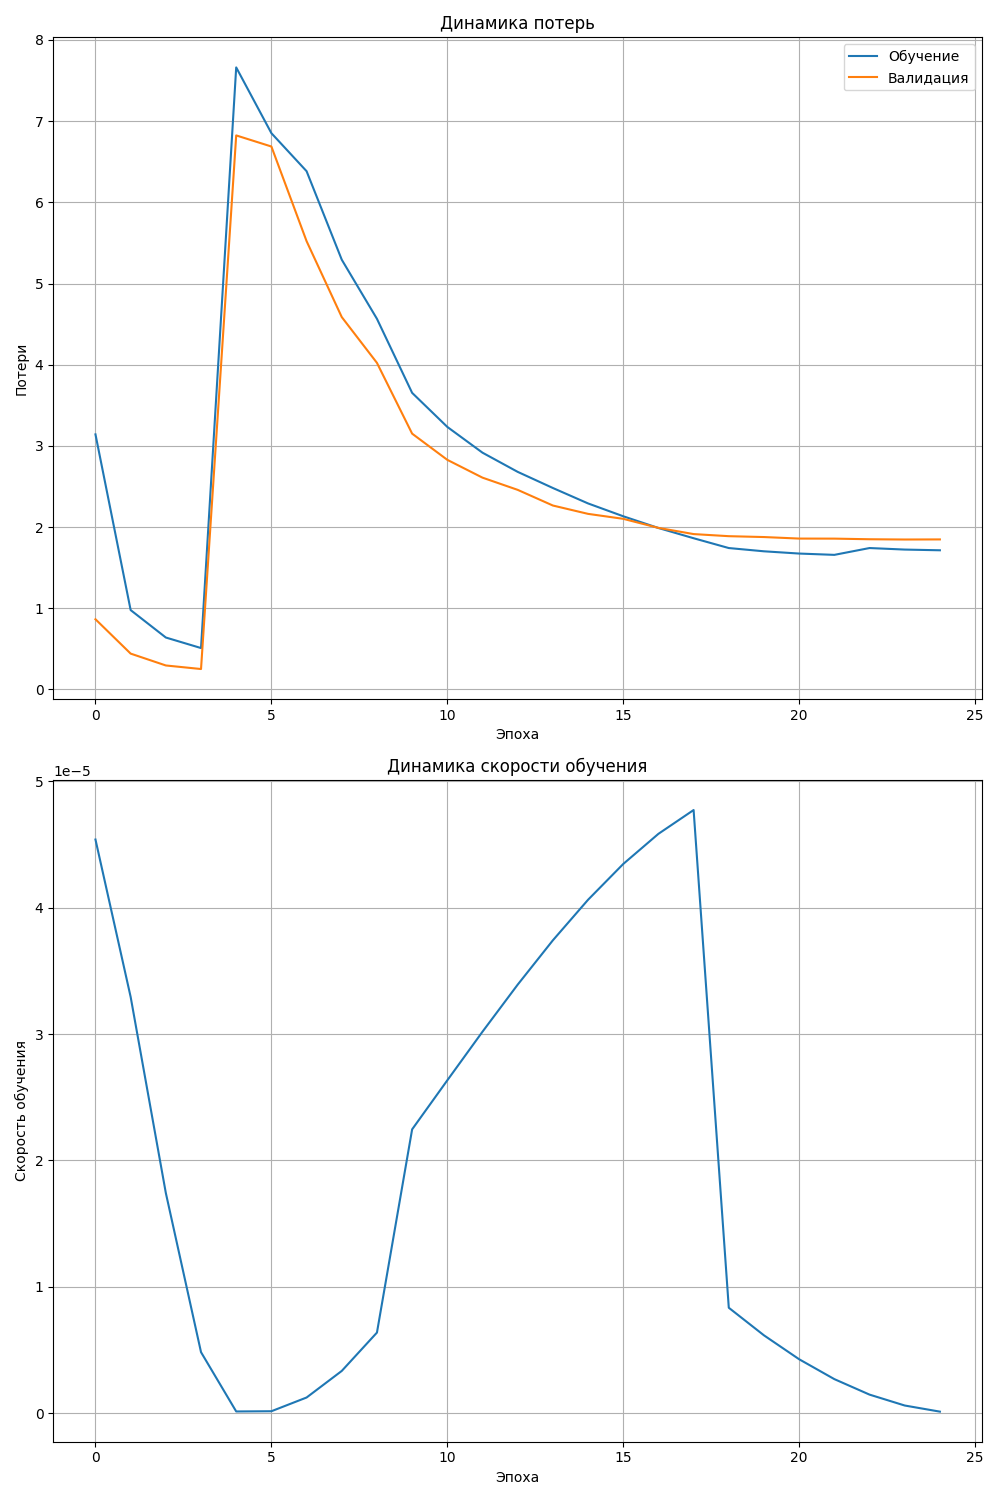
\includegraphics[width=0.8\textwidth]{metrics_epoch_25.png}
			\caption{График потерь обучения модели Donut (25 эпох).}
			\label{fig:donut_metrics_plot}
		\end{figure}
		
		\begin{table}[h!]
			\centering
			\caption{Сводка метрик обучения Donut (выборочные эпохи).}
			\label{tab:donut_metrics_summary}
			\resizebox{\textwidth}{!}{%
				\begin{tabular}{@{}lcccccc@{}}
					\toprule
					\textbf{Метрика / Эпоха} & \textbf{1} & \textbf{2} & \textbf{3} & \textbf{4} & \textbf{5} & \textbf{25} \\
					\midrule
					Train Loss & 3.1420 & 0.9779 & 0.6399 & 0.5102 & 7.6620 & 1.7144 \\
					Val Loss & 0.8649 & 0.4417 & 0.2957 & 0.2519 & 6.8244 & 1.8483 \\
					Learning Rate & 4.54e-05 & 3.29e-05 & 1.74e-05 & 4.82e-06 & 1.25e-07 & 1.11e-07 \\
					Time per Epoch (s) & 8797.71 & 8792.64 & 8793.67 & 8793.04 & 351.68 & 347.86 \\
					\bottomrule
				\end{tabular}%
			}
		\end{table}
	\end{itemize}
	
	\subsection{Метрики для детекции текста (YOLO)}
	Для оценки качества модели детекции текста YOLOv12 используются следующие стандартные метрики:
	\begin{itemize}
		\item \textbf{Precision (Точность):} Доля правильно обнаруженных текстовых областей среди всех предсказанных моделью. Высокая точность означает, что модель делает мало ложных срабатываний.
		\item \textbf{Recall (Полнота):} Доля правильно обнаруженных текстовых областей среди всех реально существующих текстовых областей в данных. Высокая полнота означает, что модель находит большинство текстовых объектов.
		\item \textbf{F1-score:} Гармоническое среднее Precision и Recall, предоставляющее сбалансированную оценку, особенно полезную при дисбалансе классов или когда важны и точность, и полнота. Рассчитывается как $2 \cdot \frac{Precision \cdot Recall}{Precision + Recall}$.
		\item \textbf{mAP (mean Average Precision):} Среднее значение Average Precision (AP) по всем классам. В нашем случае, поскольку класс один ("текст"), mAP@0.5 означает AP при пороге IoU = 0.5, а mAP@0.5:0.95 означает среднее AP по диапазону порогов IoU от 0.5 до 0.95 с шагом 0.05. Это основная метрика для оценки общей производительности моделей детекции объектов.
		\item \textbf{IoU (Intersection over Union):} Метрика, измеряющая степень перекрытия предсказанной ограничивающей рамки с истинной. Рассчитывается как площадь пересечения рамок, деленная на площадь их объединения. Используется для определения, является ли предсказание верным (True Positive).
	\end{itemize}
	
	Визуализация результатов работы модели и кривых метрик представлена ниже.
	
	\begin{figure}[h!]
		\centering
		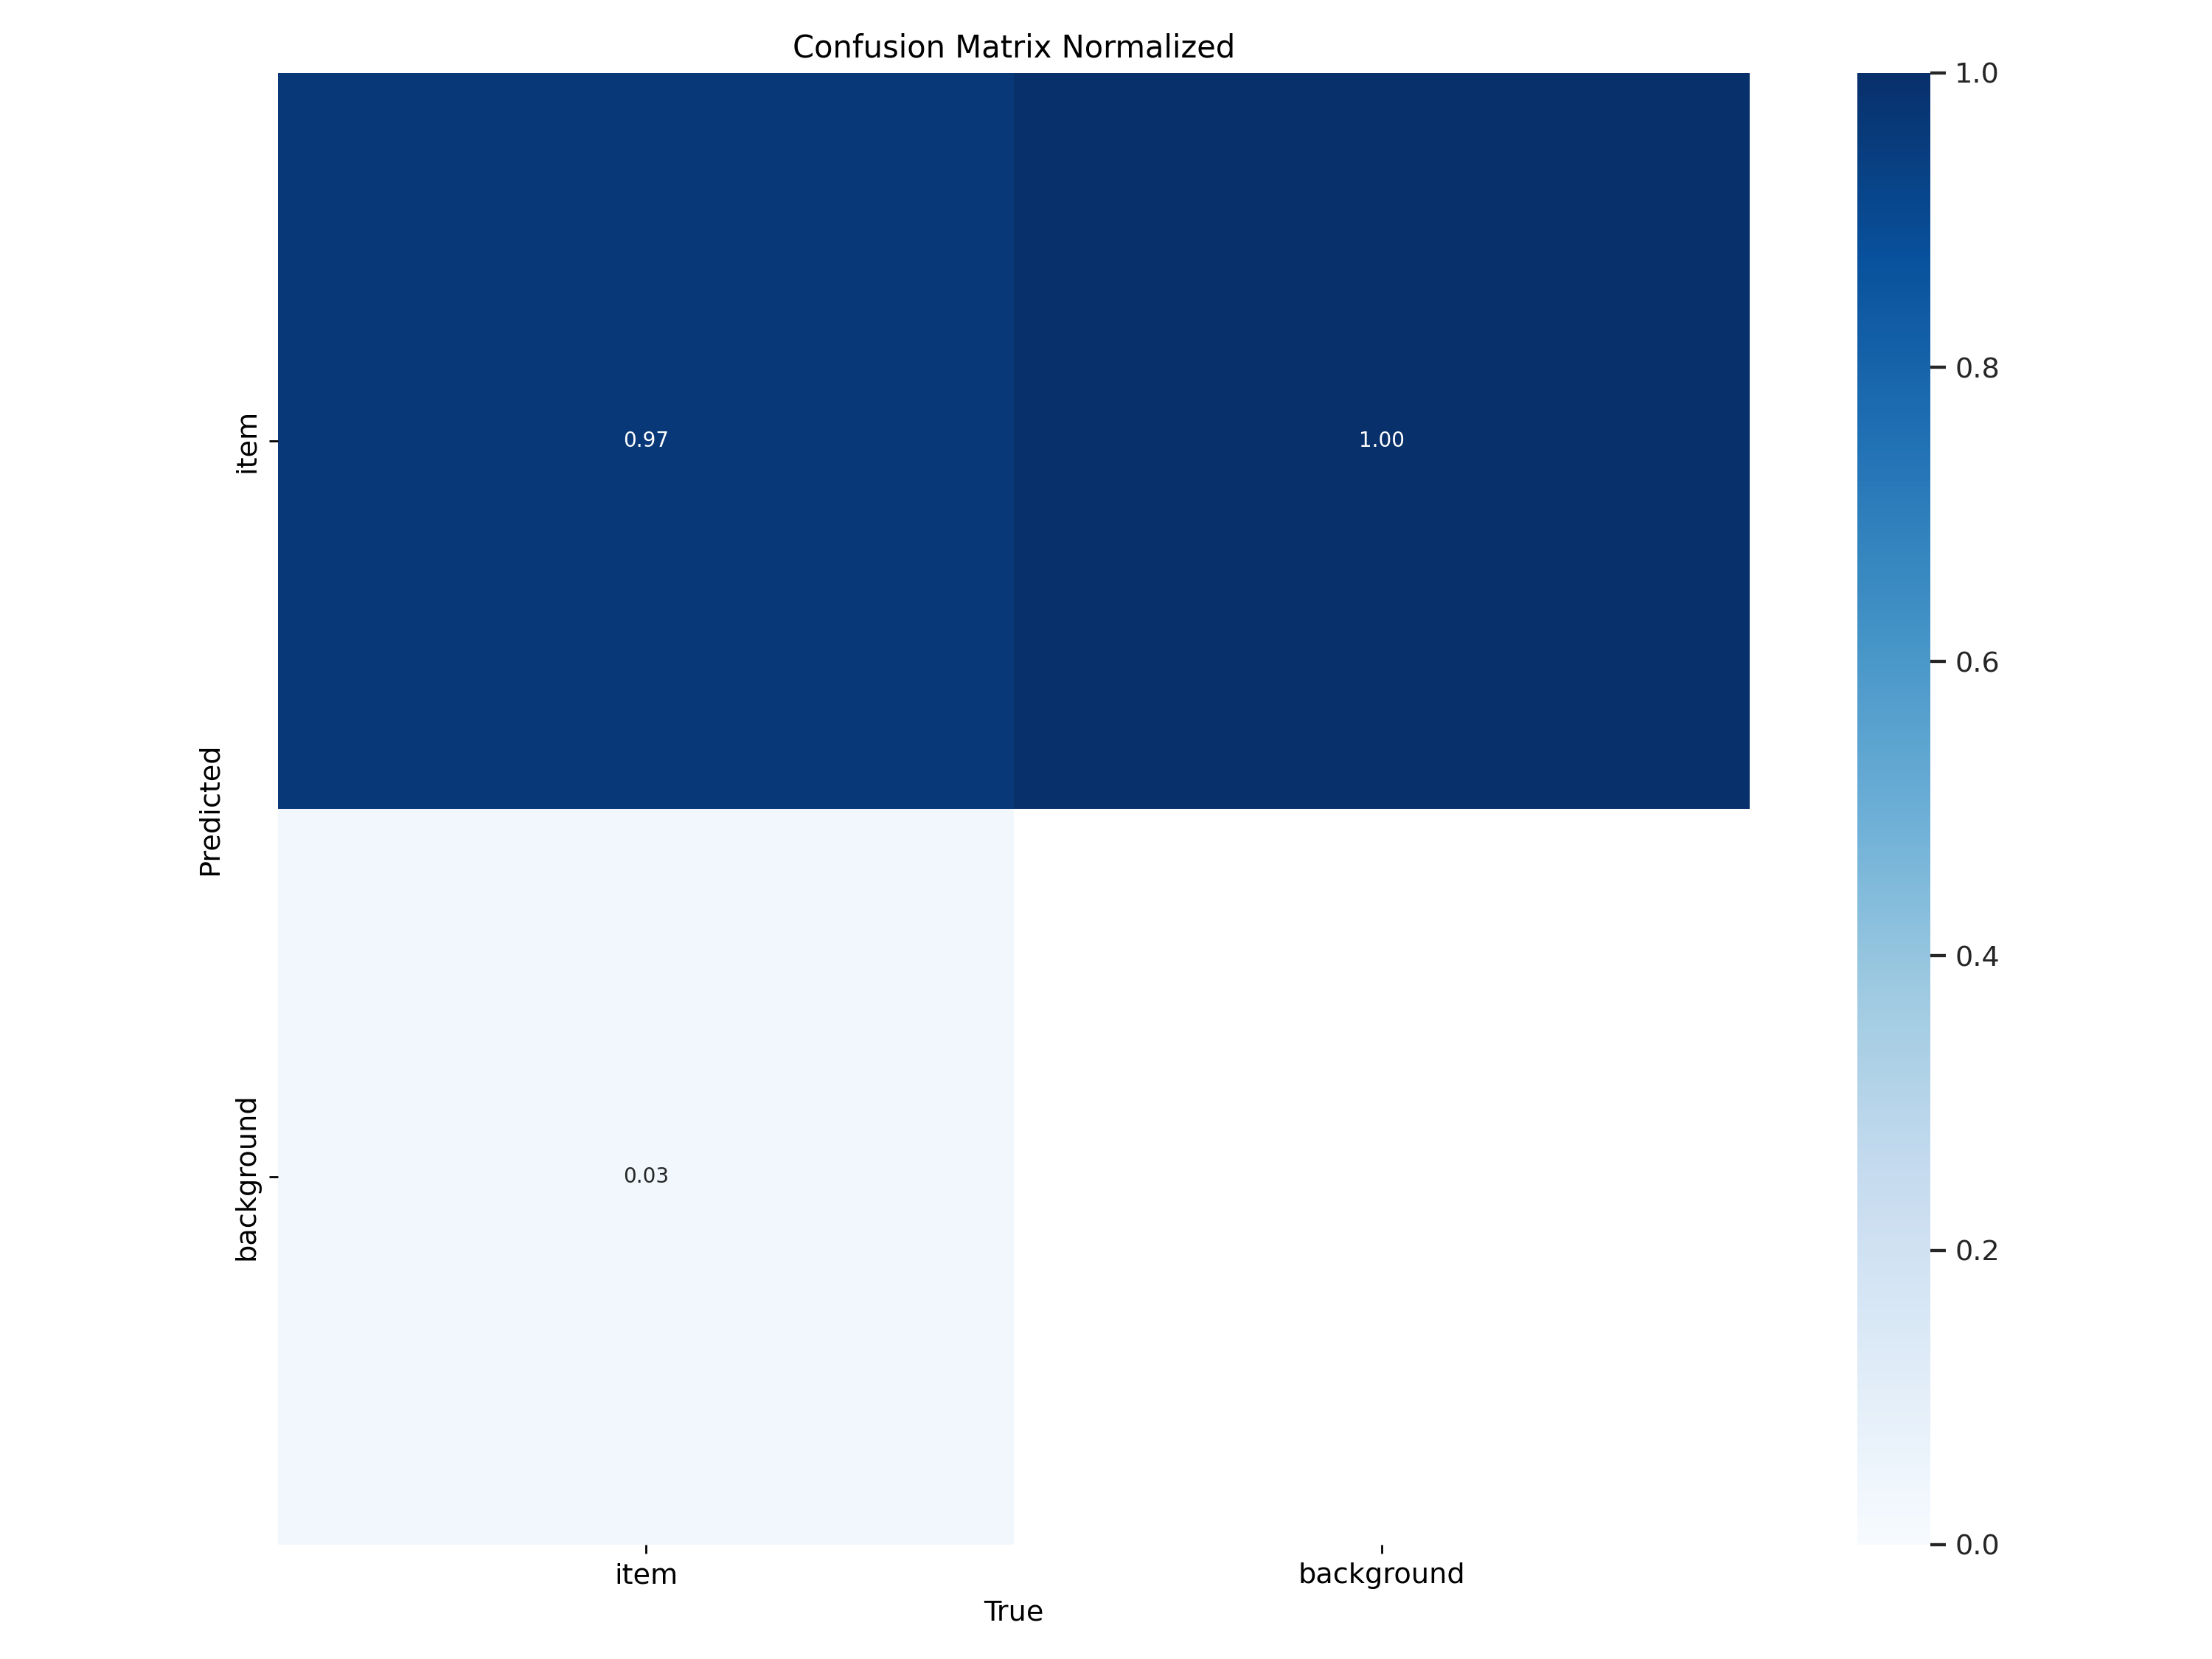
\includegraphics[width=0.7\textwidth]{confusion_matrix_normalized.png}
		\caption{Нормализованная матрица ошибок для модели детекции YOLOv12.}
		\label{fig:yolo_confusion_matrix}
	\end{figure}
	
	\begin{figure}[h!]
		\centering
		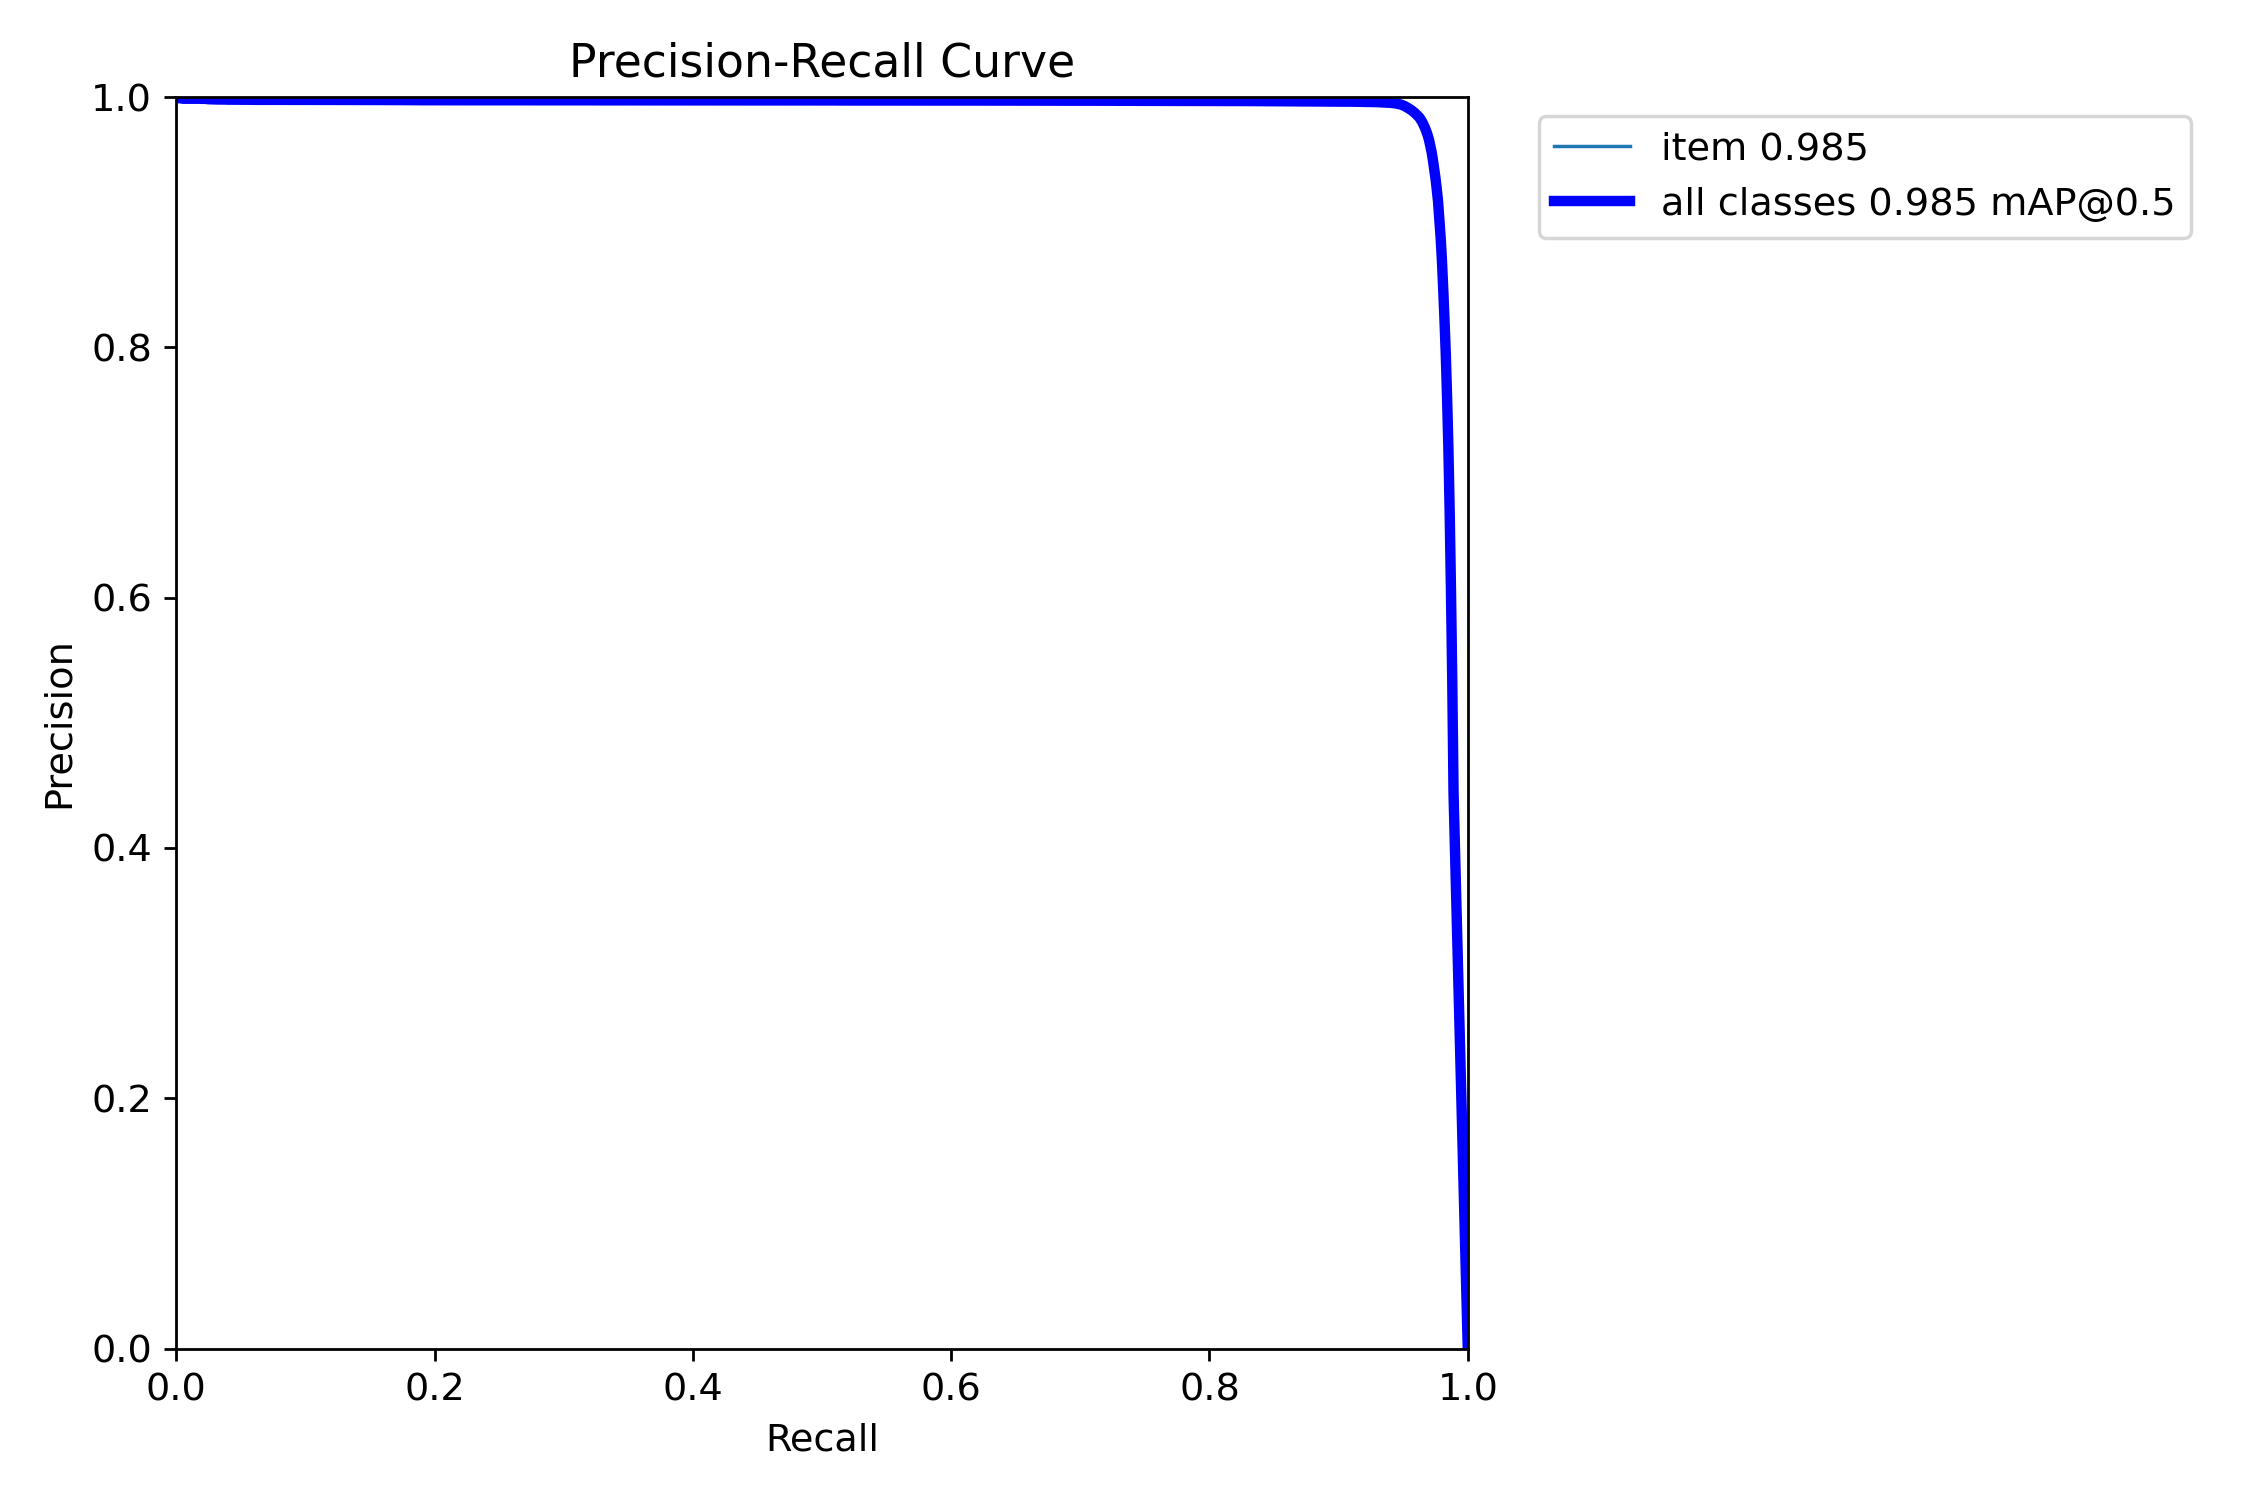
\includegraphics[width=0.7\textwidth]{PR_curve.png}
		\caption{Кривая Precision-Recall (Точность-Полнота) для модели YOLOv12.}
		\label{fig:yolo_pr_curve}
	\end{figure}
	
	\begin{figure}[h!]
		\centering
		\begin{subfigure}[b]{0.48\textwidth}
			\centering
			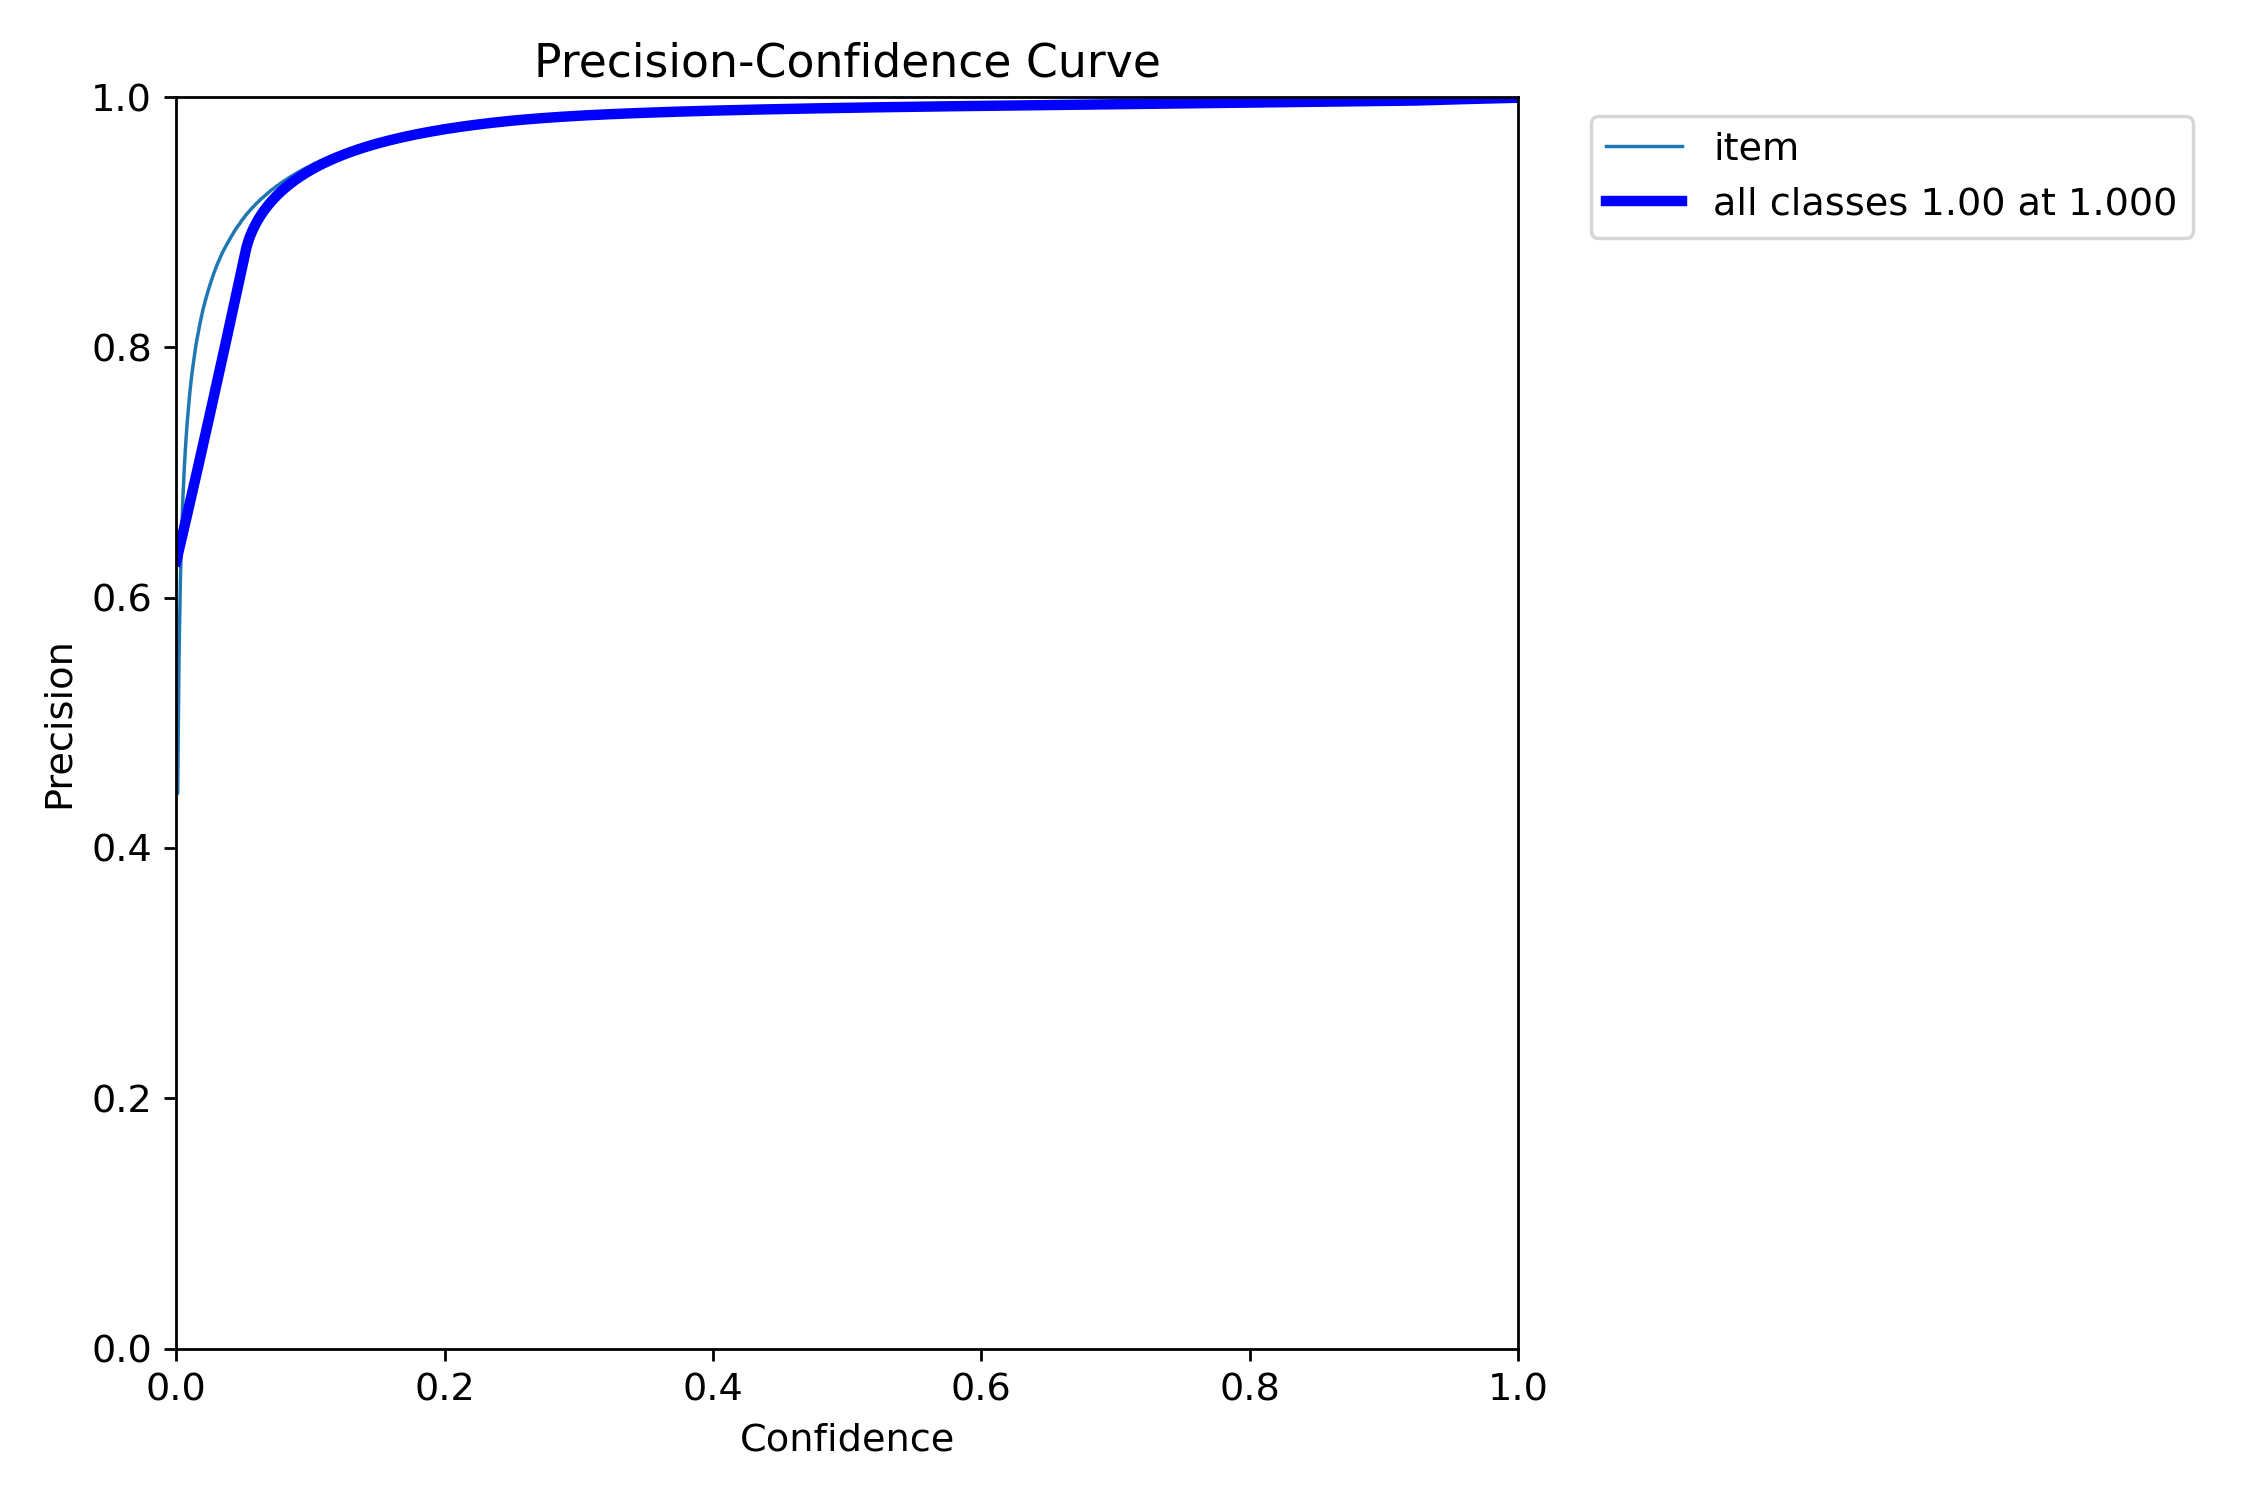
\includegraphics[width=\textwidth]{P_curve.png}
			\caption{Кривая Precision.}
			\label{fig:yolo_p_curve}
		\end{subfigure}
		\hfill
		\begin{subfigure}[b]{0.48\textwidth}
			\centering
			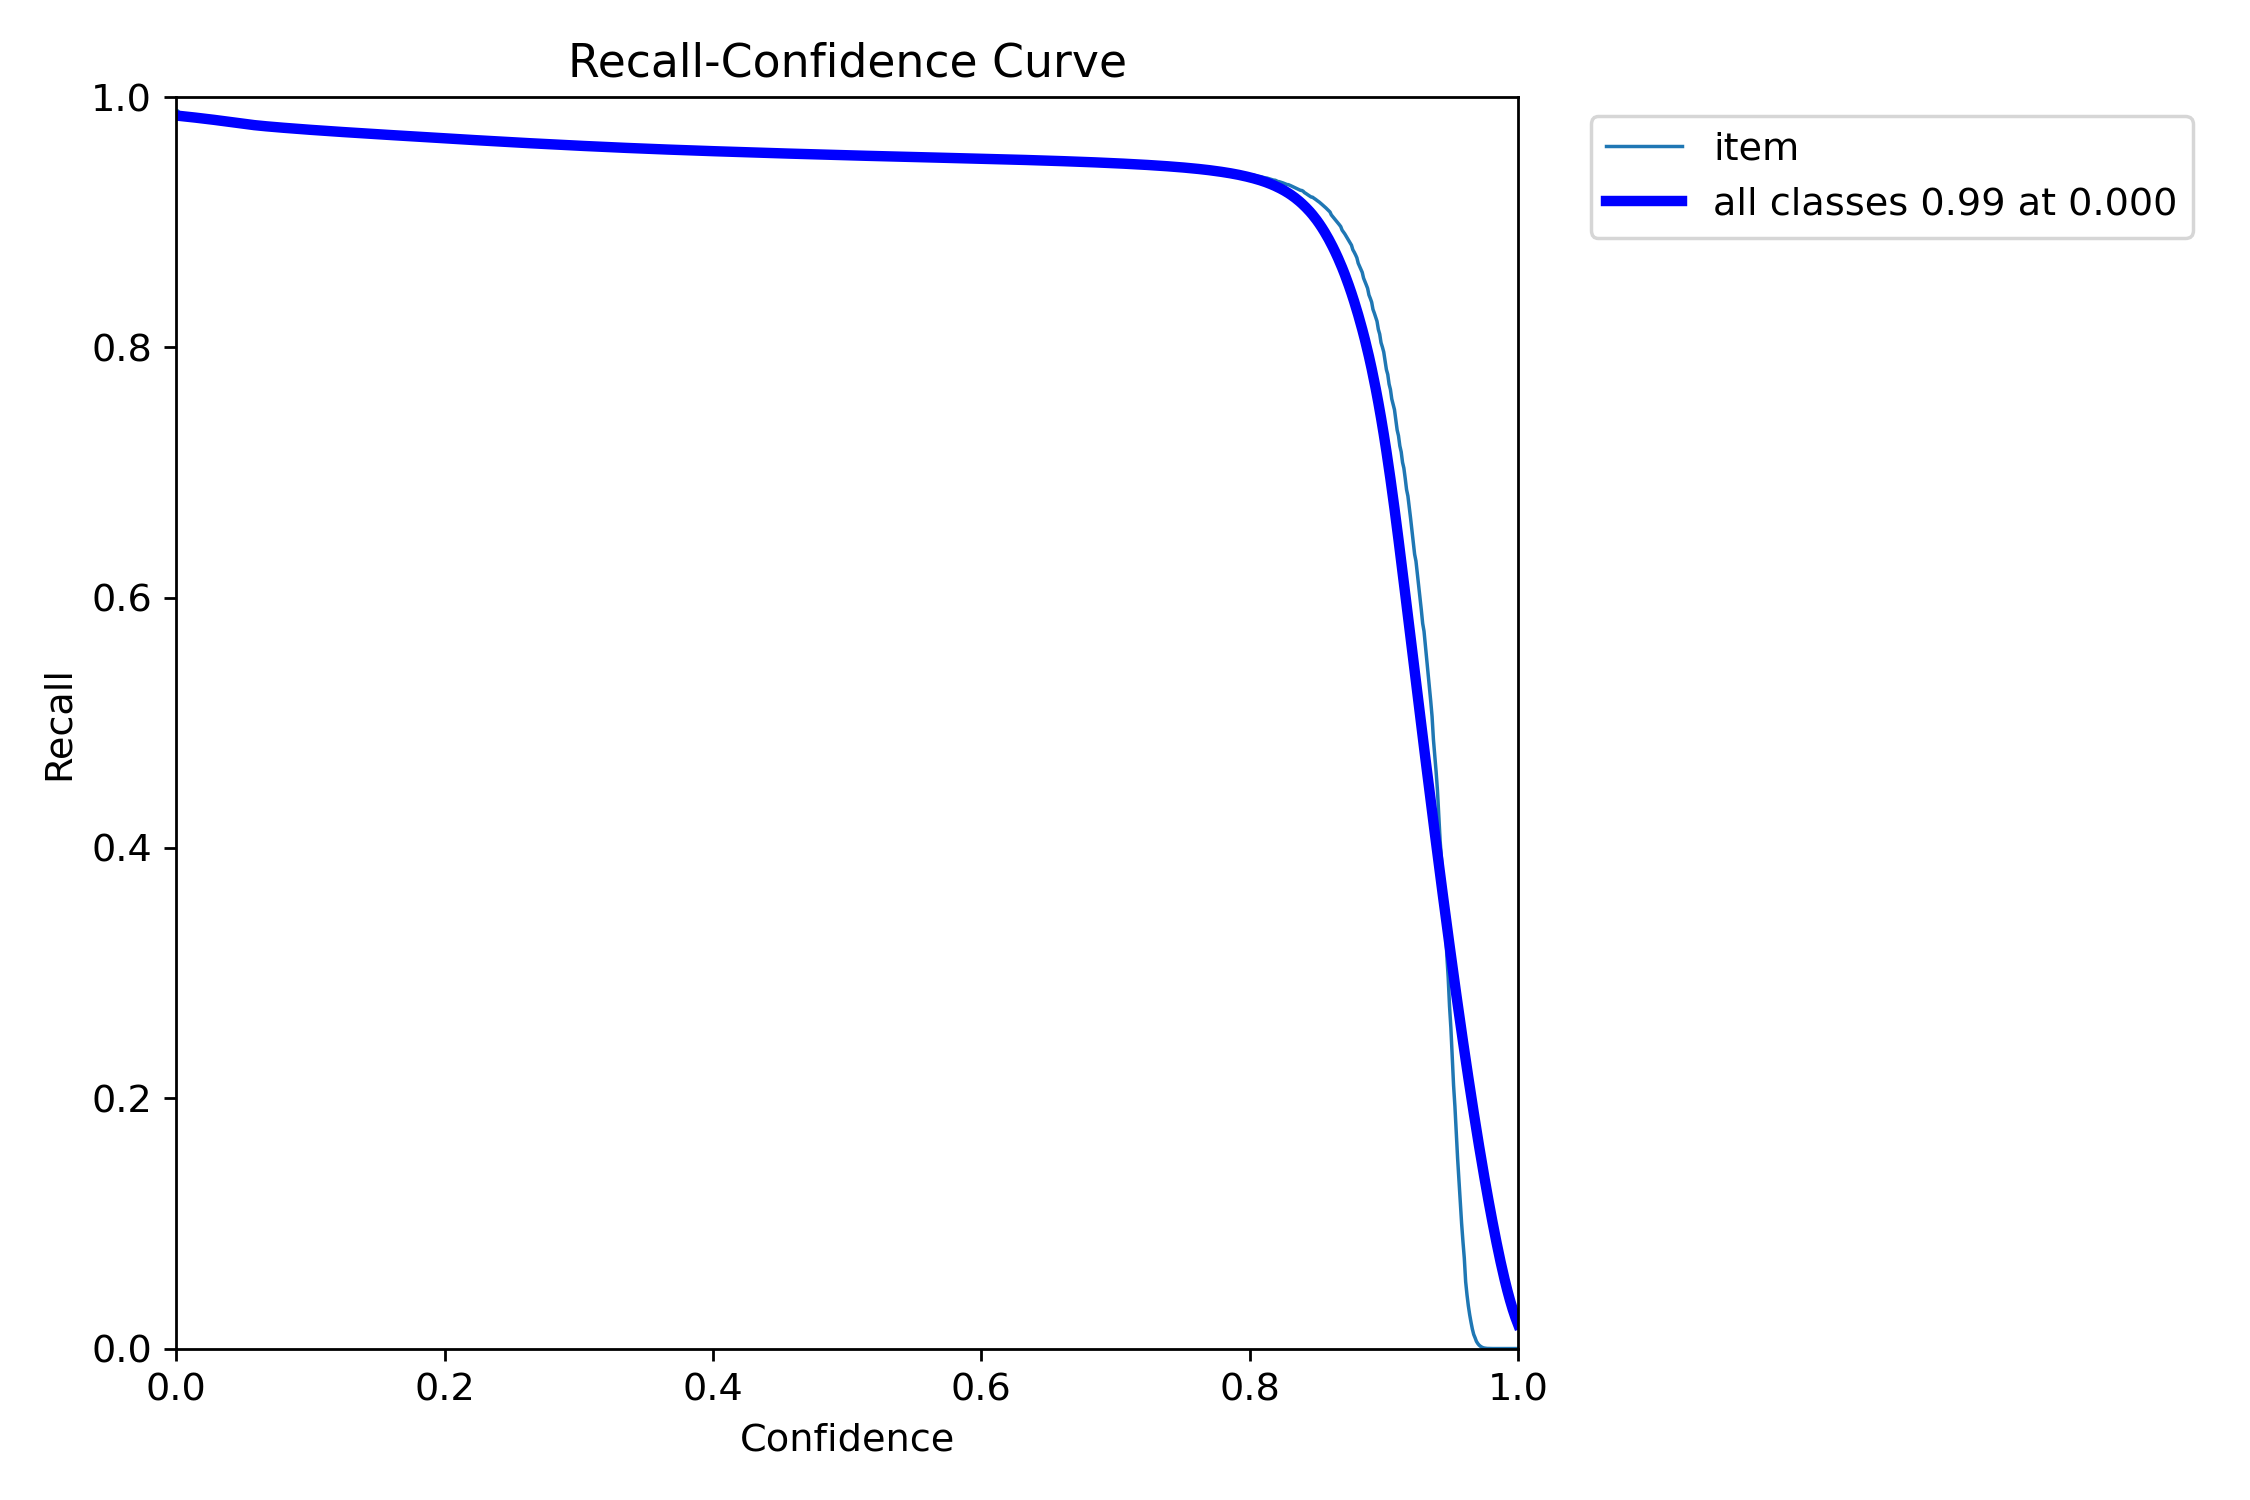
\includegraphics[width=\textwidth]{R_curve.png}
			\caption{Кривая Recall.}
			\label{fig:yolo_r_curve}
		\end{subfigure}
		\caption{Кривые Precision и Recall в зависимости от порога уверенности (confidence) для модели YOLOv12.}
		\label{fig:yolo_p_r_curves}
	\end{figure}
	
	\begin{figure}[h!]
		\centering
		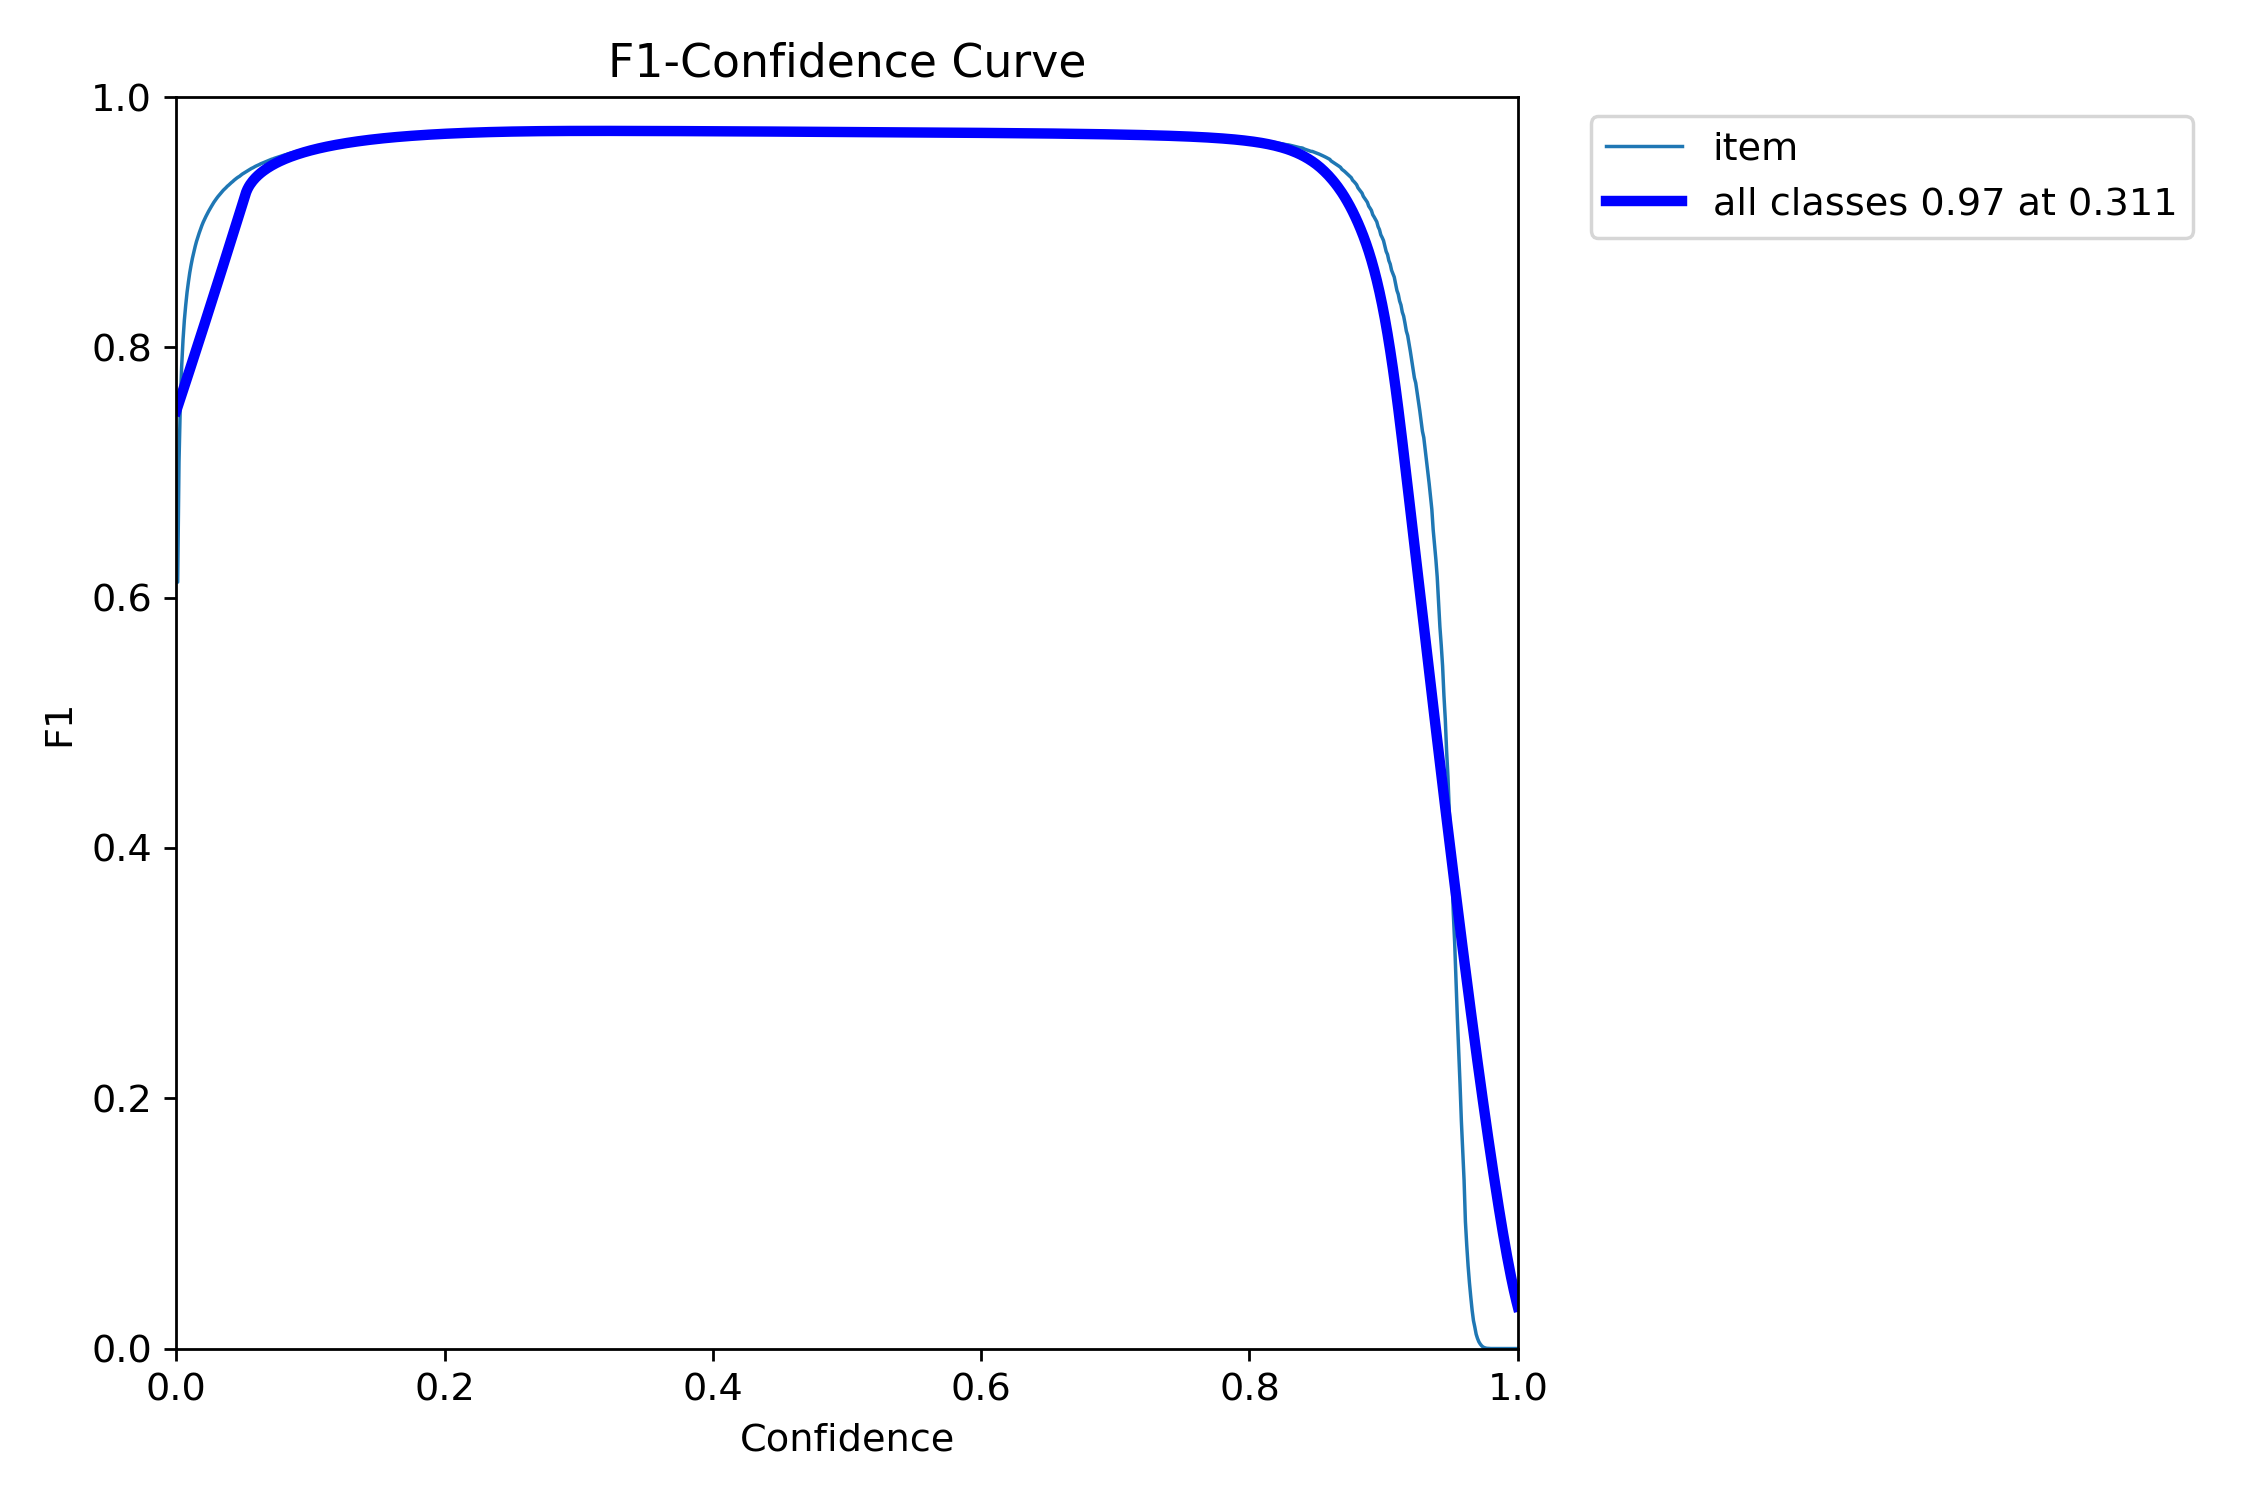
\includegraphics[width=0.7\textwidth]{F1_curve.png}
		\caption{Кривая F1-score в зависимости от порога уверенности (confidence) для модели YOLOv12.}
		\label{fig:yolo_f1_curve}
	\end{figure}
	
	\begin{figure}[h!]
		\centering
		\begin{subfigure}[b]{0.48\textwidth}
			\centering
			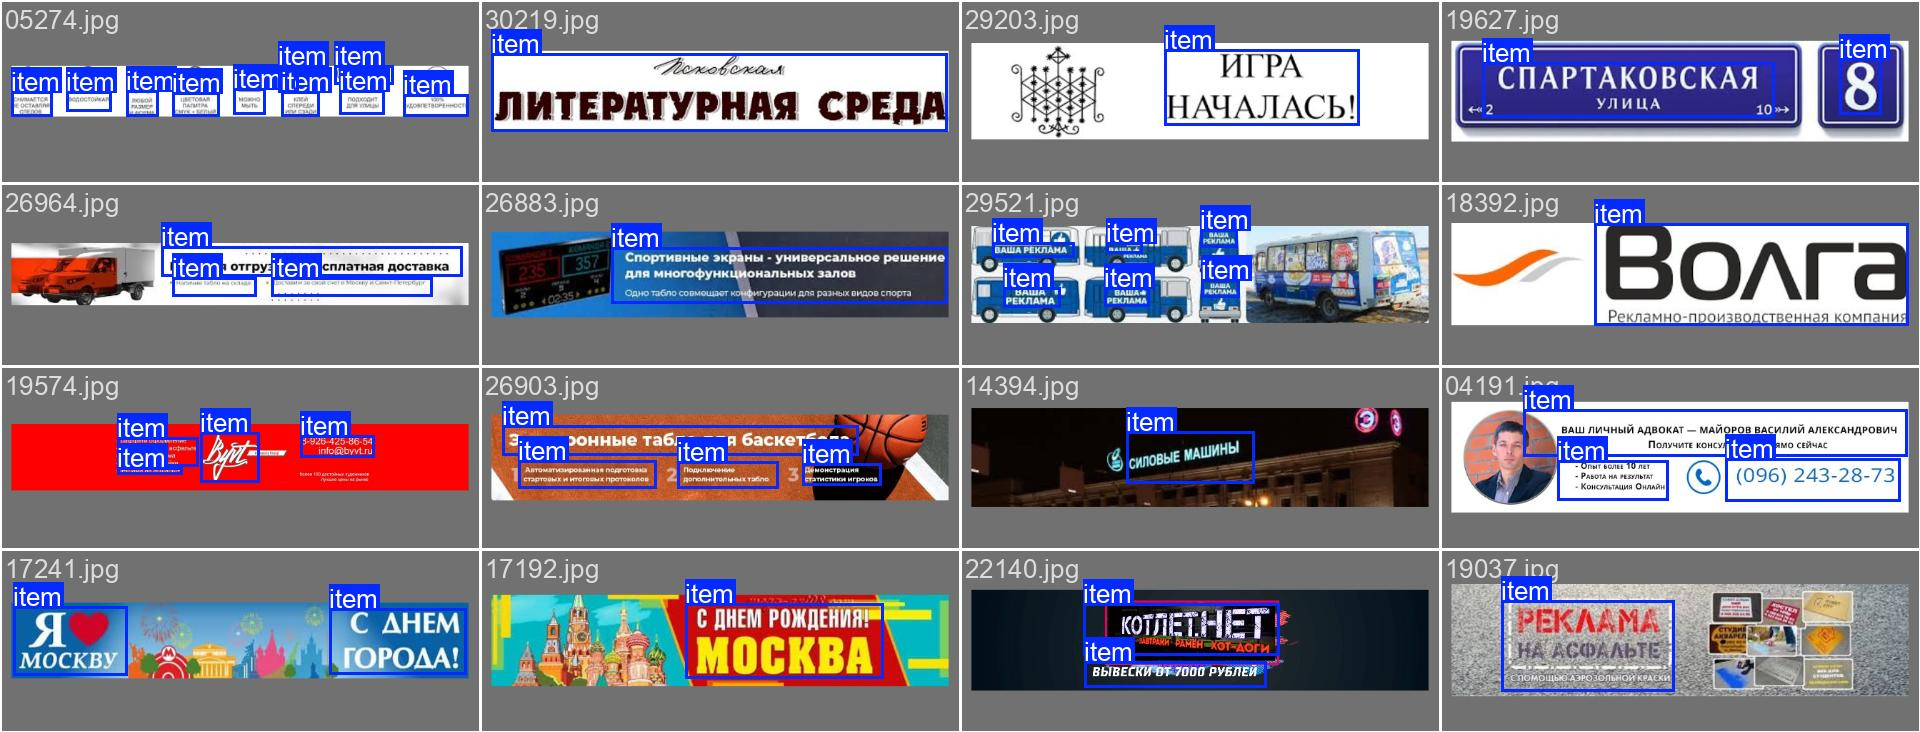
\includegraphics[width=\textwidth]{val_batch0_labels.jpg}
			\caption{Пример разметки (ground truth) из валидационного набора.}
			\label{fig:yolo_val_labels}
		\end{subfigure}
		\hfill
		\begin{subfigure}[b]{0.48\textwidth}
			\centering
			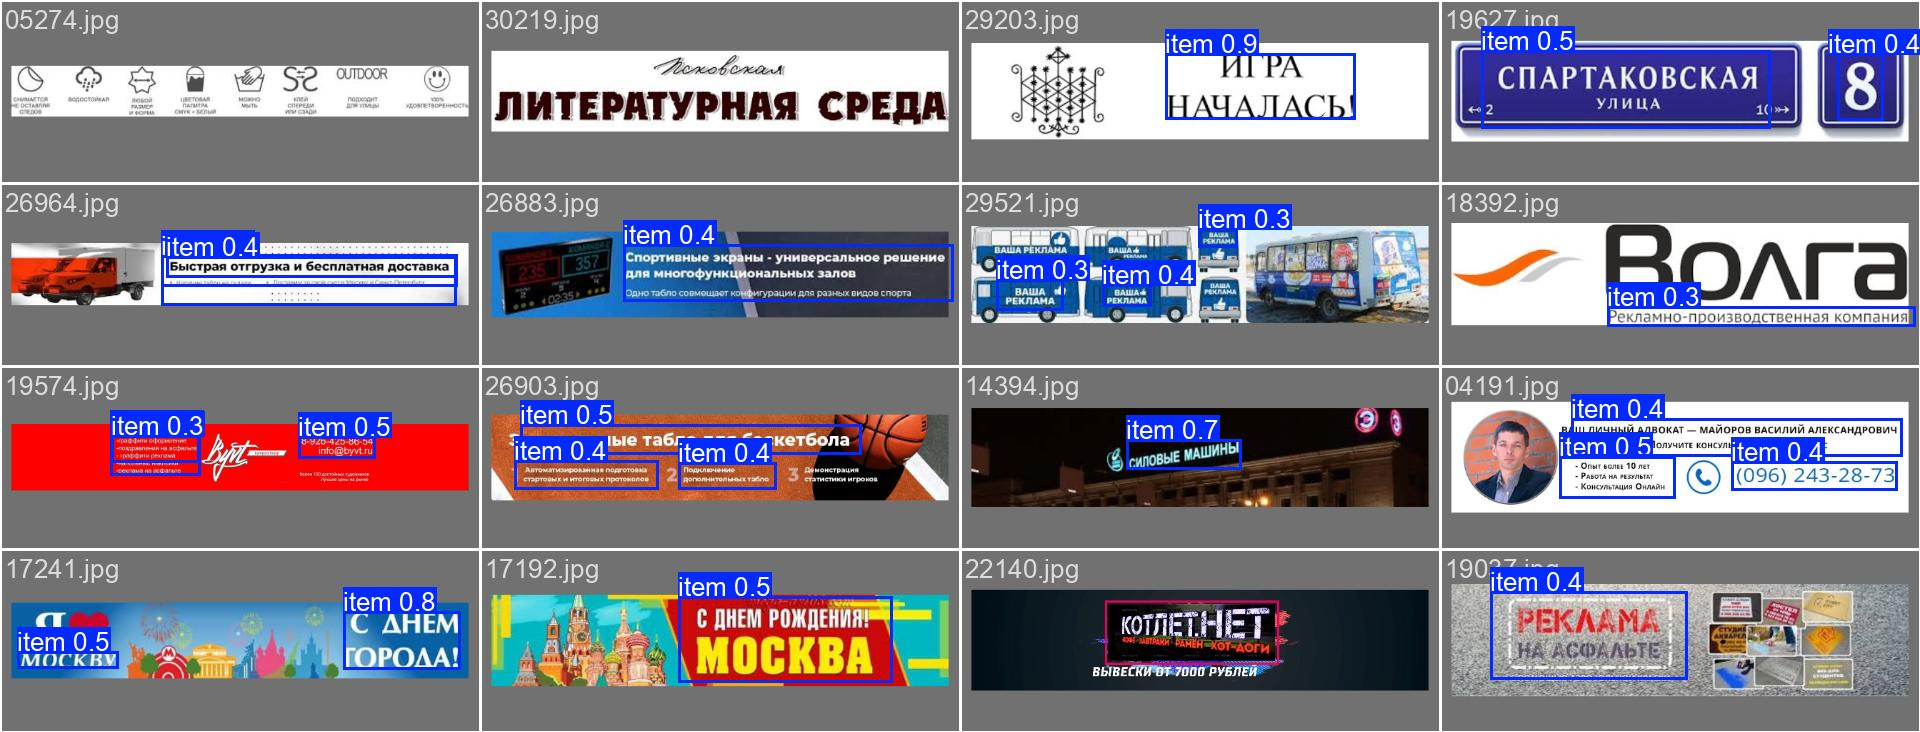
\includegraphics[width=\textwidth]{val_batch0_pred.jpg}
			\caption{Предсказания модели YOLOv12 для соответствующего изображения.}
			\label{fig:yolo_val_pred}
		\end{subfigure}
		\caption{Визуальный пример работы модели YOLOv12: истинная разметка и предсказания модели на изображении из валидационного набора.}
		\label{fig:yolo_val_examples}
	\end{figure}
	
	
	\subsection{Метрики для распознавания текста (TrOCR, Donut)}	
	Мы использовали метрику \textbf{Character Similarity Score (Коэффициент символьного сходства)}. Эта метрика рассчитывается на основе нормализованного расстояния редактирования (edit distance), такого как расстояние Левенштейна.
	Нормализованное расстояние редактирования (\texttt{normalized\_edit\_distance}) представляет собой долю ошибок (0.0 для идентичных строк, 1.0 для полностью различных строк при одинаковой длине, или если одна из строк пуста). Соответственно, \textbf{Character Similarity Score} рассчитывается как \texttt{1.0 - normalized\_edit\_distance}. Таким образом:
	\begin{itemize}
		\item Значение \textbf{1.0} означает идеальное совпадение предсказанной строки с эталонной на уровне символов.
		\item Значение, близкое к \textbf{0.0}, указывает на очень низкое сходство между предсказанием и эталоном.
	\end{itemize}
	
	На рисунке \ref{fig:char_similarity_dist} представлено распределение значений Character Similarity Score для результатов распознавания одной из наших моделей (Donut). Это позволяет визуально оценить, какая доля предсказаний имеет высокий уровень сходства с эталонами, а какая — низкий. Идеальное распределение было бы сконцентрировано вблизи значения 1.0.
	
	\begin{figure}[h!]
		\centering
		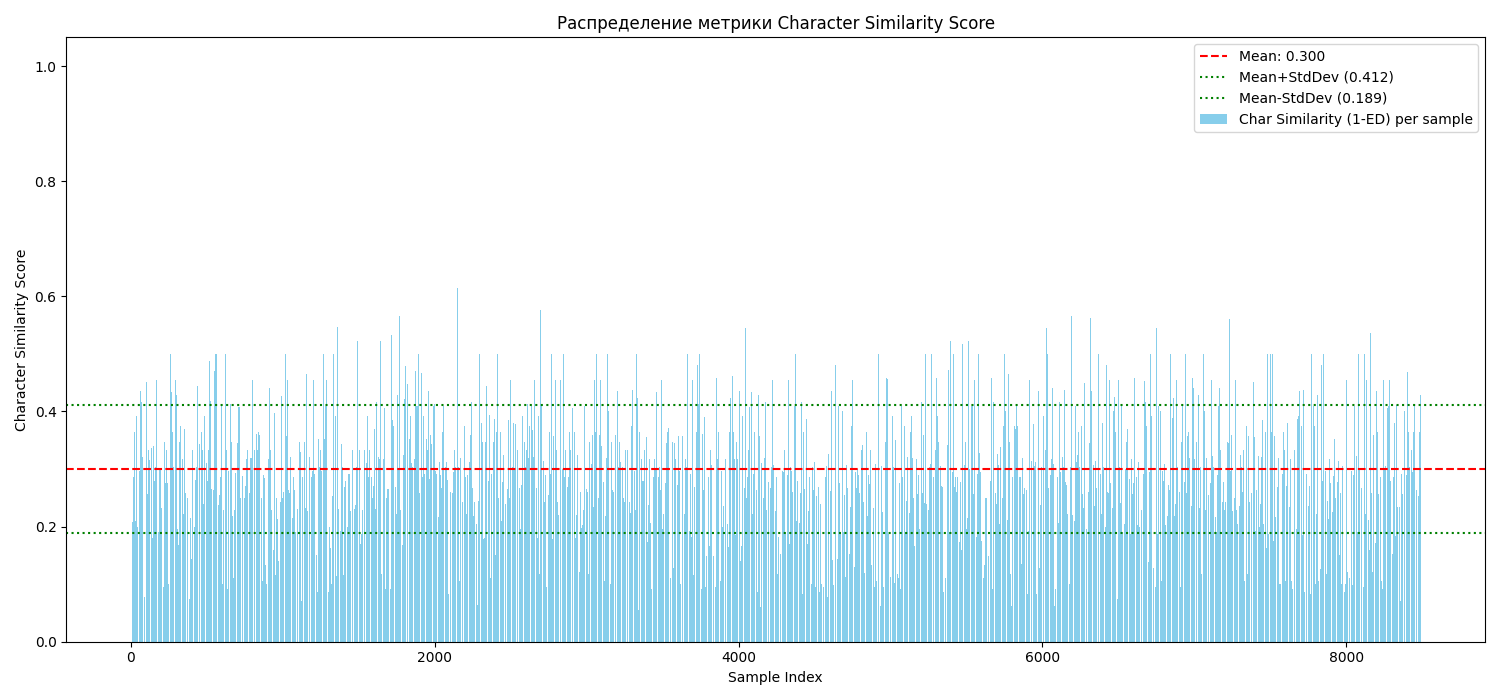
\includegraphics[width=0.8\textwidth]{char_similarity_distribution.png}
		\caption{Распределение коэффициента символьного сходства (Character Similarity Score) для результатов распознавания текста.}
		\label{fig:char_similarity_dist}
	\end{figure}
		
	
	\section{Развертывание и демонстрация}
	Развернутое решение FrameReader состоит из нескольких компонентов: бэкенд-сервера (ветка $server$), фронтенд-приложения (ветка $client$) и сервера для инференса моделей (ветка $triton-server$).
	
	\subsection{Использование в продакшене (Сервер инференса)}
	Для развертывания обученных моделей в продакшене используется NVIDIA Triton Inference Server в связке с Ray Serve. Такой подход обеспечивает высокую производительность, масштабируемость и гибкость инференса. Модели экспортируются в оптимизированный формат, такой как TensorRT engine, для достижения максимальной производительности.
	
	\textbf{Архитектура сервера инференса:}
	Архитектура построена на следующих ключевых компонентах:
	\begin{itemize}
		\item \textbf{NVIDIA Triton Inference Server:} Открытая платформа для инференса, поддерживающая различные фреймворки (TensorFlow, PyTorch, ONNX Runtime, TensorRT) и обеспечивающая высокую пропускную способность и низкую задержку.
		\item \textbf{Ray Serve:} Библиотека для развертывания моделей и сервисов на Ray, которая легко интегрируется с Triton Server для управления инференсом.
	\end{itemize}
	
	\textbf{Поддерживаемые модели и их реализация в Triton Server:}
	\begin{itemize}
		\item \textbf{YOLO:} Используется для детекции текстовых областей (предположительно YOLOv12). Модель загружается в Triton Server в оптимизированном формате (например, TensorRT engine).
		\item \textbf{Donut:} Используется для оптического распознавания символов (OCR). Для этой модели реализован \textbf{кастомный движок TensorRT инференса}, что позволяет адаптировать стандартный инференс Donut для работы с TensorRT и достичь максимальной производительности.
	\end{itemize}
	Модели для Triton Server располагаются в директории $triton-server/models/$. Каждая модель имеет свою поддиректорию с файлом конфигурации $config.pbtxt$ и версиями модели (например, $1/$).
	
	\subsection{API и интерфейсы}
	\subsubsection{API сервера инференса}
	Triton Server и Ray Serve предоставляют несколько эндпоинтов для взаимодействия:
	\begin{itemize}
		\item \textbf{Ray Serve API:} Эндпоинты для инференса моделей, такие как $http://localhost:8000/yolo$ и $http://localhost:8000/donut$. Также доступен эндпоинт для проверки состояния $http://localhost:8000/health$.
		\item \textbf{Метрики и мониторинг:} Эндпоинт для метрик $http://localhost:8002/metrics$ и дашборд Ray $http://localhost:8265$.
	\end{itemize}
	Пример запроса к Ray Serve для инференса YOLO:
	\begin{lstlisting}[language=python, caption=Пример запроса к Ray Serve для YOLO]
		import requests
		import base64
		
		with open("image.jpg", "rb") as f:
		image_data = base64.b64encode(f.read()).decode()
		
		response = requests.post(
		"http://localhost:8000/yolo",
		json={"image": image_data}
		)
		
		print(response.json())
	\end{lstlisting}
	Поддерживается как основной (main) API, так и потоковый (streaming) API для получения результатов обработки.
	
	\subsubsection{API Бэкенда}
	Бэкенд-сервер (ветка $server$) предоставляет REST API и WebSocket API для взаимодействия с клиентским приложением.
	\begin{itemize}
		\item \textbf{REST API:} Используется для управления сессиями, например, создание сессии через POST-запрос на $http://localhost:8000/api/video_sessions$.
		\item \textbf{WebSocket API:} Используется для потоковой передачи аннотаций видео и получения результатов в реальном времени, например, через эндпоинт $ws://localhost:8000/ws/video_recognition/{session_id}$.
	\end{itemize}
	
	\subsection{Компоненты системы}
	\subsubsection{Бэкенд (Server)}
	Ветка $server$ является основным бэкендом проекта, реализующим логику работы с базой данных, трекинг видео, распознавание текста и интеграцию с Triton Server.
	
	\textbf{Основные функции и архитектура бэкенда:}
	\begin{itemize}
		\item \textbf{Трекинг видео:} Обработка видеопотоков для детекции текстовых областей.
		\item \textbf{Распознавание текста (OCR):} Извлечение и распознавание текста из выделенных областей.
		\item \textbf{Управление данными:} Хранение информации о пользователях, сессиях обработки видео и результатах распознавания в базе данных MySQL.
		\item \textbf{API:} Предоставление RESTful API и WebSocket API на основе FastAPI.
		\item \textbf{Интеграция с Triton Server} для выполнения моделей.
	\end{itemize}
	
	\textbf{Структура базы данных:}
	MySQL используется для хранения данных о пользователях, сессиях и результатах. Структура включает таблицы для сессий видео ($video_sessions$) и распознанных текстах ($annotation_frame$). Пример таблицы для пользователей:
	\begin{lstlisting}[language=sql, caption=Пример таблицы для пользователей в MySQL]
		CREATE TABLE IF NOT EXISTS users (
		id INT AUTO_INCREMENT PRIMARY KEY,
		username VARCHAR(255) NOT NULL UNIQUE,
		email VARCHAR(255) NOT NULL UNIQUE,
		created_at TIMESTAMP DEFAULT CURRENT_TIMESTAMP
		);
	\end{lstlisting}
	
	\subsection{Демонстрация}
	\href{https://github.com/Prischli-Drink-Coffee/FrameReader?tab=readme-ov-file#%D0%B4%D0%B5%D0%BC%D0%BE%D0%BD%D1%81%D1%82%D1%80%D0%B0%D1%86%D0%B8%D1%8F-%D1%80%D0%B0%D0%B1%D0%BE%D1%82%D1%8B}{Демо приложения}
	
	\section{Выводы и перспективы}
	\subsection{Основные результаты работы}
	Проект FrameReader демонстрирует комплексный подход к задаче извлечения и распознавания текста из видео. Разработанное решение объединяет передовые модели компьютерного зрения (YOLO, TrOCR, Donut) с эффективной инфраструктурой развертывания (Triton Server, Ray Serve) и удобным пользовательским интерфейсом. Это позволяет автоматизировать процесс анализа видеоконтента и получать структурированную текстовую информацию.
	
	\subsection{Нерешенные проблемы}
	Несмотря на достигнутые результаты, существуют аспекты, требующие дальнейшего внимания:
	\begin{itemize}
		\item Точность распознавания текста недостаточна хороша и может варьироваться для очень специфичных шрифтов, низкого качества видео или сложных условий съемки.
		\item Обработка рукописного текста в видео на данный момент не реализована.
		\item Оптимизация производительности для обработки видеопотоков сверхвысокого разрешения в реальном времени может потребовать дополнительных исследований.
	\end{itemize}
	
	\subsection{Планы масштабирования}
	\begin{itemize}
		\item \textbf{Улучшение точности OCR:} Дальнейшее обучение моделей на более разнообразных и специфичных датасетах для русского языка, а также исследование новых архитектур.
		\item \textbf{Обработка рукописного текста:} Расширение функционала для распознавания рукописного текста в видео.
		\item \textbf{Оптимизация производительности:} Дальнейшая оптимизация моделей и инфраструктуры для обработки видео в реальном времени с еще большей скоростью.
		\item \textbf{Расширение функционала:} Добавление возможностей для поиска по распознанному тексту, аннотирования видео, экспорта результатов в различные форматы.
		\item \textbf{Мультиязычность:} Поддержка распознавания текста на нескольких языках.
	\end{itemize}
	
\end{document}